\documentclass[12pt,oneside]{book}

\usepackage{CUThesis2025}
\usepackage{lscape}
\usepackage{amsmath,amssymb}
\usepackage{graphicx}
\usepackage{booktabs}
\usepackage{caption}
\usepackage{subcaption}
\usepackage{tikz}
\usetikzlibrary{arrows.meta,positioning,shapes.geometric}

%% --- THESIS METADATA --- %%
\title{From Measured Pore-Scale Operators to Network-Level Prediction in a Structured Belousov--Zhabotinsky Reactor}
\author{Srivijayesh Venugopal}
\date{September 2026}
\faculty{\FEAS}
\course{Computational Fluid Dynamics}
\degree{MSc}
\supervisor{Prof. Weisi Guo}
\academicyear{2025--2026}
\copyrightyear{2026}

\begin{document}

\maketitle
\frontmatter

%% --- ABSTRACT --- %%
\begin{abstract}
This thesis treats a structured Belousov--Zhabotinsky (BZ) reaction--diffusion medium as the micro-scale picture inside a macro-scale porous chemical reactor.
The internal geometry of such a reactor, a network of pores connected by narrow throats, is too fine to resolve in a full continuum simulation.
Instead, the pores and throats are abstracted as nodes and edges of a graph, and the local pulse-traffic rules at each element are measured in controlled two-dimensional simulations of the light-sensitive Oregonator model.

A verified explicit finite-difference solver is used in a black-box protocol to isolate and measure four native operators: pulse transmission along a straight throat, refractory-limited frequency response, two-input inhibition at a T-junction, and anisotropic routing under a tilted diffusion tensor.
The measurements are translated into an event-driven graph simulator in which nodes and edges carry the measured transit times, refractory times, and inhibition windows.
The graph simulator is validated against full partial-differential-equation (PDE) solutions for an inhibition gate, a priority router, and a shared-control two-path gate.

The work shows that network-level pulse routing can be predicted from micro-scale transfer functions, but only when junction geometry is accounted for.
A three-dimensional inhibition gate and a one-way diode pilot are reported as boundary experiments: the 3D gate works after geometry correction, while the diode shows that a simple asymmetric wall or static light barrier is insufficient for robust rectification.
The thesis closes by identifying the remaining steps toward trained porous chemical processors and molecular-communication substrates.
\end{abstract}

\begin{keywords}
physical neural networks, reaction-diffusion computing, excitable media,
Belousov--Zhabotinsky reaction, Oregonator model, analog computation,
molecular communication, porous media, pore-network model, neuromorphic engineering
\end{keywords}

%% --- ACKNOWLEDGEMENTS --- %%
\chapter*{Acknowledgements}
I would like to thank my supervisors, Professor Weisi Guo, Professor Panagiotis Takis Tsoutsanis, and Professor Tamas Josza for their guidance and support throughout this research project.

%% --- FRONT MATTER --- %%
{
\clearpage
\singlespacing
\tableofcontents
\clearpage
\listoffigures
\clearpage
\listoftables
}

\begin{listofabbreviations}
    \abbrev{RD}{Reaction--Diffusion}
    \abbrev{BZ}{Belousov--Zhabotinsky}
    \abbrev{CRN}{Chemical Reaction Network}
    \abbrev{RNCRN}{Recurrent Neural Chemical Reaction Network}
    \abbrev{PNN}{Physical Neural Network}
    \abbrev{RNN}{Recurrent Neural Network}
    \abbrev{ODE}{Ordinary Differential Equation}
    \abbrev{PDE}{Partial Differential Equation}
    \abbrev{BC}{Boundary Condition}
    \abbrev{FDTD}{Finite-Difference Time-Domain}
    \abbrev{CFD}{Computational Fluid Dynamics}
\end{listofabbreviations}

%% --- MAIN MATTER --- %%
\mainmatter
\pagestyle{fancy}
\fancyhead[L]{\nouppercase{\leftmark}}
\fancyhead[R]{\nouppercase{\rightmark}}

\chapter{Introduction}
\label{chap:introduction}
% Chapter: Introduction
% Porous BZ reactor as a structured reaction-diffusion computing substrate

\section{Background and Motivation}
\label{sec:background}

Digital computers move data between memory and processor for every operation, and this von Neumann bottleneck costs energy and latency at every arithmetic step.
As machine-learning workloads grow, there is increasing interest in using the physics of a material to compute directly, without clocked digital arithmetic.
In such physical neural networks, inputs are encoded as physical excitations, the medium transforms them through its own dynamics, and outputs are read from probes.
Computation is continuous in time and parallel across space, with the medium's structure acting as the network's weights.
Demonstrations in optics, mechanics, and electronics show that this approach can work in practice \cite{lin2018alloptical, wright2022deep, hughes2019wave}.

This project starts from a simple question: what happens inside a porous chemical reactor when a pulse of reagent is injected at one face?
The reactor is a solid scaffold saturated with a reacting fluid; its internal geometry is a maze of pores joined by narrow throats.
A chemical excitation introduced at one pore will travel through the fluid, split at junctions, collide with other excitations, and possibly reach output locations on another face.
If the local rules that govern this traffic are known, the reactor can be treated as a programmable analog computer whose program is written into the pore geometry and the spatial distribution of chemical properties.

Making this precise requires two things: a medium rich enough to support directed pulse traffic, and a systematic way to describe what a given arrangement of it computes.
This thesis builds the case for one answer and tests it.
\refSec{sec:lit_pnn} reviews the physical-neural-network idea, \refSec{sec:lit_chemical} the chemical and excitable-media route to computation, and \refSec{sec:lit_bz} the Belousov--Zhabotinsky reaction and Oregonator model as the practical realisation.
\refSec{sec:lit_synthesis} draws these threads into the research gap, from which the aim and objectives follow.

\section{Physical Neural Networks}
\label{sec:lit_pnn}

A physical neural network is a material or device whose internal physical dynamics implement the operations of a neural network.
Inputs are encoded as fields or excitations, the material transforms them through its natural evolution, and outputs are read from detectors.
The appeal is that computation can occur in parallel across space and continuously in time, without the repeated memory transfers that dominate digital inference.

Optical systems provide the most prominent demonstrations.
Silva \etal showed that a metamaterial slab can perform mathematical operations such as spatial differentiation and integration on an incident electromagnetic field \cite{silva2014performing}.
Shen \etal demonstrated a coherent nanophotonic circuit that implements a deep neural network for image classification entirely in the optical domain \cite{shen2017deep}.
Lin \etal extended this to diffractive deep neural networks, in which successive phase masks modulate free-space propagation so that the outgoing intensity pattern encodes the classification result \cite{lin2018alloptical}.
The geometry of the masks or scatterers serves as the trainable weights.

Mechanical and thermal analogs offer complementary physical bases.
Stern \etal demonstrated supervised learning through physical changes in a mechanical network of springs and masses \cite{stern2020supervised}, and later developed a broader framework for learning in physical networks \cite{stern2021physical}.
Wright \etal extended the idea to deep architectures by chaining multiple physical systems and training them with backpropagation through differentiable simulations \cite{wright2022deep}.
Thermal analog computing has been proposed for matrix-vector multiplication using inverse-designed metastructures \cite{silva2026thermal}.
These demonstrations prove that the PNN concept is not restricted to any one physics.

A unifying theoretical perspective was provided by Hughes \etal, who showed that linear wave propagation can be written as an analog recurrent neural network \cite{hughes2019wave}.
In this view, the wave field at each time step is the hidden state, and the evolution operator is a sparse linear recurrence whose coefficients depend on local material properties.
McMahon reviewed the broader trend of nonlinear computation with linear systems and argued that such approaches are becoming practical for specialised tasks \cite{mcmahon2024nonlinear}.

The present work adopts the same stance---the physical field is the computational state and the material distribution is the trainable parameter set---but moves from linear wave physics to a nonlinear, excitable chemical medium.
The propagating quantity is a self-sustaining chemical pulse rather than a decaying or superposing wave.
This situates the work within molecular communication: the substrate is a fluid channel whose input is a spatially patterned chemical excitation and whose output is a measured concentration signal.
Experimental tabletop molecular communication has already demonstrated digital messages carried by chemical signals \cite{farsad2013tabletop}, and surveys identify reaction--diffusion transport as a physically realistic channel model \cite{farsad2016comprehensive}.
The present thesis treats the reaction--diffusion channel not merely as a passive link, but as a programmable analog computing substrate.

\section{Chemical and Excitable-Media Computing}
\label{sec:lit_chemical}

Computation in fluid and chemical media has a long history.
Matter itself stores and transforms information, so signals are processed by the physics of the substrate rather than by an external arithmetic unit.
The lineage runs from hydraulic analog machines to modern molecular and microfluidic systems \cite{adamatzky2019liquid}.
Demonstrated platforms include microfluidic bubble logic, in which gas bubbles carry, route, and process discrete bits through channel networks \cite{prakash2007bubble}, and self-organising chemical reaction networks that classify temporal inputs as reservoir computers \cite{baltussen2024chemical}.

Within this tradition, excitable chemical media offer a direct route to computation because their elementary phenomena map onto computational primitives.
An excitable medium has a stable rest state, a threshold for excitation, and a refractory period after excitation during which the medium cannot be re-excited.
A supra-threshold perturbation triggers a self-sustaining pulse that propagates at a characteristic speed, leaving a refractory wake.
Colliding pulses annihilate; pulses meeting a narrowing gap or high-curvature turn can be blocked \cite{courtemanche1993instabilities}.
These primitives have produced working devices: colliding-pulse logic gates, an experimental XOR gate in a reaction--diffusion medium, logical functions of structured channel junctions, and a single oscillating BZ droplet acting as a binary and fuzzy logic processor \cite{toth1995logic, steinbock1996chemical, adamatzky2002xor, adamatzky2002collision, sielewiesiuk2001logical, gorecki2009information, gentili2012chemical}.
The common feature is hand design: each gate or circuit is built geometry by geometry for one logical function.

A parallel line of research pursues trainable chemistry in well-mixed reactors, where a reaction network plays the role of a neural network with reaction rates as trainable weights.
Neural-network behaviour, universal computation, and end-to-end training have been demonstrated \cite{hjelmfelt1991chemical, magnasco1997chemical, dack2024rncrn, cherry2018scaling}, but these systems are well-mixed: all information resides in scalar concentrations, with no spatial extent.
They sacrifice exactly the spatial continuity and parallelism that structured excitable media possess natively.
The present work keeps the spatial structure and asks how it can be abstracted and predicted.

\subsection{From Isolated Gates to Composed Computing}
\label{subsec:lit_gates}

The excitable-media computing literature is rich in isolated gates but poor in composition rules.
T\'{o}th and Showalter built a chemical XOR gate in which colliding pulses annihilate in a membrane-separated reaction--diffusion medium \cite{toth1995logic}.
Steinbock \etal used a geometrically structured BZ layer to implement logic gates and a chemical diode \cite{steinbock1996chemical}.
Adamatzky explored collision-based computing in excitable media, showing how streams of wave fragments can be routed and combined to perform computation \cite{adamatzky2002collision, adamatzky2002xor}.
G\'{o}recki \etal designed specific junction geometries to obtain logic gates and information-processing devices \cite{gorecki2009information}.

What is missing is a systematic way to compose these local gates into a predictive network model.
The present thesis addresses exactly this gap: it measures local transfer functions and composes them in a fast graph-level simulator, so that candidate networks can be explored before committing to expensive continuum simulations.

\section{The Belousov--Zhabotinsky Reaction and the Oregonator Model}
\label{sec:lit_bz}

The Belousov--Zhabotinsky (BZ) reaction, the metal-ion-catalysed oxidation of an organic substrate by bromate in acidic solution, is the canonical experimental excitable chemical medium.
It oscillates spontaneously under appropriate conditions and, in thin quasi-two-dimensional layers, supports propagating oxidation waves: expanding target patterns, rotating spirals, and interacting fronts.
Its phenomenology is well characterised, its ingredients are inexpensive and handled at room temperature, and compact models reproduce its behaviour faithfully.
It is therefore the standard testbed for chemical-wave computing.

The kinetic essence is captured by the Oregonator, Field and Noyes's three-variable reduction of the detailed Field--K\"or\"os--Noyes mechanism \cite{field1974oregonator}, and by Tyson and Fife's further reduction to two variables: a fast activator and a slow recovery variable \cite{tyson1980target}.
The singular-perturbation structure of the two-variable form underlies the classic understanding of pulse propagation in excitable media \cite{tyson1988singular}.
It is the model used throughout this thesis, coupled to spatial diffusion of the activator.

A variant of particular importance for computing is the photosensitive BZ reaction, in which the ruthenium-catalysed system is inhibited by illumination.
A spatial light field then acts as a writable mask: illuminated regions slow or block wave propagation, dark regions transmit it.
Sakurai \etal exploited this to route chemical waves through optically defined channels and junctions in real time \cite{sakurai2002design}.
In the language of this thesis, the light field $\phi(x,y)$ turns the substrate into a rewritable device.

The computing-relevant phenomenology of excitable media follows from a small set of robust behaviours.
A supra-threshold perturbation triggers a pulse travelling at a characteristic speed; behind it lies a refractory zone that cannot be re-excited, setting a maximum signalling frequency.
Colliding pulses annihilate; pulses meeting a narrowing gap can be blocked \cite{courtemanche1993instabilities}.
Structure adds more: asymmetric junctions act as chemical diodes \cite{agladze1996chemical}, T-shaped junctions as band-pass filters of pulse frequency \cite{gorecka2003tshaped}, and anisotropy creates preferred propagation directions \cite{steinbock1995anisotropy}.
Propagation, refractoriness, annihilation, block, rectification, filtering, and anisotropic routing are the native instruction set this work characterises.

\subsection{Pore-Network Models of Transport}
\label{subsec:lit_pore_networks}

The graph abstraction used in this thesis is borrowed from petroleum engineering and groundwater flow, where pore-network models predict multiphase flow and transport by assigning conductances to throats and solving for pressure and saturation on the graph \cite{xiong2016review, blunt2017multiphase}.
In those models a pore is a node, a throat is an edge, and the transport law is usually linear or weakly nonlinear.
The emphasis is on effective permeability, relative permeability curves, and dispersion, not on excitable pulses.

Pore-network models have also been applied to reactive transport, where species diffuse and react inside a network of pores \cite{meakin2009modeling}.
Again, the focus is on effective reaction rates rather than on threshold-activated pulse traffic.
Excitable media on networks have been studied by coupling discrete excitable elements according to a graph topology \cite{kinouchi2006optimal}, but the local element is typically a cellular-automaton node with a hand-chosen rule, not a calibrated continuous reaction--diffusion segment.

The present work differs in two ways.
First, the local element is a continuous reaction--diffusion segment whose transfer function is extracted from PDE simulations.
Second, the graph parameters are not chosen by hand but measured, so the model is calibrated rather than assumed.

\section{Synthesis and Research Gap}
\label{sec:lit_synthesis}

The literature reviewed above establishes five points.
First, physical neural networks are a viable alternative to digital inference, with trained demonstrations in optics, mechanics, and wave physics \cite{lin2018alloptical, stern2021physical, wright2022deep, hughes2019wave}.
Second, chemical and fluid media have a long computing pedigree, from liquid computers to bubble logic and chemical reservoirs \cite{adamatzky2019liquid, prakash2007bubble, baltussen2024chemical}.
Third, excitable media support wave-collision logic, diodes, filters, and routers, both in simulation and in BZ experiments \cite{toth1995logic, steinbock1996chemical, adamatzky2002xor, agladze1996chemical, gorecka2003tshaped}.
Fourth, well-mixed chemistry is trainable in the neural-network sense, but only by abandoning the spatial continuity that makes physical substrates attractive \cite{dack2024rncrn, cherry2018scaling}.
Fifth, molecular communication research treats reaction--diffusion transport as an information channel \cite{farsad2016comprehensive, guo2021molecular}, with non-coherent detectors and polynomial-chaos methods that quantify uncertainty \cite{lin2023diversity, abbaszadeh2019uncertainty}.

What is missing is a systematic way to move from the micro-scale physics inside a porous reactor to a predictive model of network-level pulse traffic.
Existing excitable-media work demonstrates isolated gates in ad hoc geometries; trainable-CRN work achieves learning but in a spaceless setting; and the physical-neural-network framework has not been carried into excitable chemical media arranged as a porous network.
Nobody has treated a structured BZ-type substrate as a set of local pore-scale operators, measured those operators in controlled two-dimensional simulations, and composed them into a fast graph-level predictor of pulse traffic.
This thesis addresses that gap.

\section{Research Aim}
\label{sec:aim}

The aim of this project is to characterise the local pulse-traffic rules inside a structured reaction--diffusion excitable medium and to show that they can be composed into a predictive pore-network model of a larger porous reactor.
Rather than asking whether such a medium can compute, the work maps out what it does natively at the pore scale, and how those local rules combine at the network scale.

\section{Research Objectives}
\label{sec:objectives}

To achieve this aim, the following objectives were set:

\begin{enumerate}
    \item Formulate the two-variable reaction--diffusion model for a two-dimensional domain, extended with structured boundaries, a spatial light-suppression field $\phi(x,y)$, and a spatially varying anisotropic diffusion tensor as substrate knobs.
    \item Implement an explicit finite-difference solver for this model and verify it against known BZ phenomenology and manufactured solutions.
    \item Design a black-box characterisation protocol in which the substrate is stimulated with pulses at input ports and its response is recorded at probe locations.
    \item Measure the native pore-scale transfer functions: channel pulse transmission, refractory-limited frequency response, two-input inhibition at a T-junction, and anisotropic routing.
    \item Build an event-driven graph simulator from the measured operators and validate it against full PDE solutions for simple networks.
    \item Identify the conditions under which the micro-scale operators transfer to three-dimensional pore geometries, and the limitations of the approach.
\end{enumerate}

\section{Scope and Delimitations}
\label{sec:scope}

In scope:
\begin{itemize}
    \item Two-dimensional reaction--diffusion dynamics in the Oregonator model, the chemically grounded reduction of the BZ mechanism.
    \item Explicit finite-difference time integration on a regular Cartesian grid.
    \item Three substrate parameterisations: wall geometry, the light-suppression field $\phi(x,y)$, and an anisotropic diffusion tensor field.
    \item Pulse-based input/output: localised activator perturbations as inputs, time-series probe recordings as outputs.
    \item A graph simulator built from measured local operators and validated against PDE solutions.
    \item Boundary three-dimensional tests that probe the transferability of the micro-scale operators.
\end{itemize}

Out of scope:
\begin{itemize}
    \item Full three-dimensional porous-medium simulations at the scale of a laboratory reactor.
    \item Experimental realisation or wet-lab validation.
    \item End-to-end training of a pore-network for a large computational task.
    \item Detailed comparison with acoustic, thermal, or well-mixed chemical alternatives; the starting point is the BZ reaction--diffusion medium.
\end{itemize}

The thesis is organised as follows.
\refChap{chap:porous} introduces the porous-reactor picture and the pore-network graph abstraction.
\refChap{chap:methodology} presents the Oregonator model, the finite-difference solver, and the graph-simulator construction.
\refChap{chap:results} reports the measured pore-scale operators and the graph-level validations.
\refChap{chap:conclusions} summarises the contributions, limitations, and next steps.


\chapter{From Porous Media to Pore-Network Graphs}
\label{chap:porous}
% Chapter: From Porous Media to Pore-Network Graphs

\section{The Porous Reactor Picture}
\label{sec:porous_picture}

Consider a macroscopic block of porous solid saturated with a reacting fluid.
The solid matrix occupies most of the volume; the remaining void space is a connected network of pores joined by narrow throats.
When a chemical excitation is injected at one face of the block, it enters the pore network as a pulse of concentration and propagates through the fluid.
At each throat the pulse travels at a speed set by the local chemistry and geometry; at each junction it may split, merge, annihilate with another pulse, or be blocked by refractory residue from a previous pulse.
The output is read as a concentration signal at probes on another face.

This is the physical picture that motivates the thesis.
The internal geometry is too fine to resolve in a full three-dimensional continuum simulation of a laboratory-scale block, and the connectivity is usually unknown.
The central move is therefore to abstract the pore space as a graph: bulbous pores become nodes and narrow throats become edges.
The fluid dynamics inside each element are replaced by measured transfer functions, and the network-level traffic is predicted by composing those functions.

The same abstraction is common in petroleum engineering and groundwater flow, where pore-network models predict multiphase flow and transport by assigning conductances to throats and solving for pressure and saturation on the graph \cite{xiong2016review, blunt2017multiphase}.
What changes here is the physics: the transported quantity is not a passive scalar carried by pressure-driven flow, but a self-sustaining excitation pulse whose existence depends on the local reaction--diffusion state.
The conductance analogue is a pulse transfer function, and the nodes carry memory in the form of refractory time.

\section{Why Two-Dimensional Controlled Simulations}
\label{sec:porous_why2d}

A real porous reactor is three-dimensional, so why study two-dimensional channels?
The answer is control.
In a thin quasi-two-dimensional layer of the photosensitive BZ reaction, a projected light mask defines the suppression field $\phi(x,y)$ everywhere in the domain.
The local kinetic parameters are therefore known and uniform across the layer, and the pulse-traffic rules can be isolated and measured.
In a three-dimensional bulk, absorption and scattering make the interior light field unknown, so the local kinetics would be uncontrolled.

Two-dimensional simulations are thus the controlled micro-scale limit of the three-dimensional porous problem.
They provide the local operators from which a three-dimensional pore-network model can later be calibrated once a volumetric illumination strategy is chosen.
The results in this thesis are therefore not a toy model; they are the micro-scale calibration layer that any predictive porous-medium description must rest on.

\section{Pore-Network Graph Abstraction}
\label{sec:porous_graph}

The graph abstraction is straightforward.
A pore is represented by a node; a throat by a directed or undirected edge.
Each edge carries a transit time, the time for a pulse to travel the throat length at the measured pulse speed.
Each node carries a refractory time, the interval after a pulse arrives during which the node will ignore further pulses.
Some nodes also carry an inhibition window: two pulses arriving within this window annihilate.
Finally, a routing table at each node decides which incoming edges feed which outgoing edges, encoding the junction topology.

This abstraction reduces a continuous PDE problem to a discrete event simulation.
It is fast enough to explore candidate pore networks in milliseconds, before committing to an expensive PDE simulation.
Its validity is the main question of the thesis.

\section{Local Operators}
\label{sec:porous_operators}

Four local operators are measured in the two-dimensional simulations reported in \refChap{chap:results}:

\begin{itemize}
    \item \textbf{Wire:} a straight throat transmits a pulse at a fixed speed with little attenuation.
    \item \textbf{Low-pass filter:} a throat drops pulses that arrive faster than the refractory time permits.
    \item \textbf{Inhibition:} at a T-junction, a pulse on one arm can block a pulse on another arm if it arrives within a short window.
    \item \textbf{Anisotropic routing:} a tilted diffusion tensor steers pulses along preferred directions, introducing path-dependent delays.
\end{itemize}

These four operators are sufficient to build a simple graph simulator.
More complex behaviours, such as one-way diodes or frequency-selective band-pass filters, are discussed in the literature but are not included as validated primitives here.
A diode pilot reported in \refSec{sec:res_diode} shows that a simple asymmetric wall geometry or static light barrier does not give robust rectification in the present parameter regime, so the diode is left as an open problem.

\section{Related Work on Pore-Network Models of Transport}
\label{sec:porous_related}

Pore-network models have been used for reactive transport, where species diffuse and react inside a network of pores \cite{xiong2016review, meakin2009modeling}.
The emphasis in that literature is on effective reaction rates and dispersion, not on excitable pulses.
Excitable media on networks have also been studied, usually by coupling discrete excitable elements according to a graph topology \cite{kinouchi2006optimal}.
The present work differs in two ways.
First, the local element is a continuous reaction--diffusion segment, not a discrete cellular-automaton node.
Second, the graph parameters are not chosen by hand but extracted from PDE simulations, so the model is calibrated rather than assumed.

The closest conceptual precedent is the idea of extracting discrete circuit rules from continuous excitable media.
Gorecki \etal designed specific junction geometries to obtain logic gates and information processing devices \cite{gorecki2009information}, and Adamatzky demonstrated collision-based computing in structured BZ media \cite{adamatzky2002collision}.
Those works build one geometry for one function.
This thesis builds a general composition framework: measure the local rules, put them in a graph simulator, and validate the composition against PDE solutions.


\chapter{Methods}
\label{chap:methodology}
% Chapter: Methods (porous reframe)

\section{Overview}
\label{sec:meth_overview}

The methodology follows a characterise-before-train philosophy: before asking how a structured excitable medium might be optimised for a computational task, we first measure, in a controlled and reproducible way, what the unoptimised medium already does.
It has four layers.

The model layer describes the BZ medium by the two-variable Tyson--Fife Oregonator, extended with substrate knobs that act as candidate weights: wall geometry, a light-suppression field, and an anisotropic diffusion tensor.
The solver layer is an explicit finite-difference scheme with adaptive reaction subcycling, verified against known excitable-media phenomenology and convergence-tested in space and time.
The protocol layer is a black-box characterisation: the substrate is stimulated at defined input ports and its response recorded at fixed probes, yielding transfer functions rather than snapshots.
The composition layer translates the measured transfer functions into an event-driven graph simulator and validates it against full PDE solutions.

\section{The Oregonator Model}
\label{sec:meth_oregonator}

\subsection{Two-Variable Reduction}
\label{sec:meth_oregonator_2var}

The chemical basis of the substrate is the BZ reaction, modelled by the two-variable Tyson--Fife reduction of the Oregonator introduced in \refSec{sec:lit_bz} \cite{field1974oregonator, tyson1980target}.
In the scaled Tyson--Fife form used throughout this thesis, the kinetics are
\begin{equation}
\frac{\partial u}{\partial t} = \frac{1}{\varepsilon}\left[\,u - u^{2} - \left(f v + \phi\right)\frac{u - q}{u + q}\,\right] + \nabla\!\cdot\!\left(\mathbf{D}\,\nabla u\right),
\label{eq:oregonator_u}
\end{equation}
\begin{equation}
\frac{\partial v}{\partial t} = u - v + D_{v}\,\nabla^{2} v,
\label{eq:oregonator_v}
\end{equation}
where $u$ is the scaled activator concentration, $v$ the scaled oxidised catalyst concentration, and $\phi$ the illumination in the photosensitive ruthenium-catalysed variant \cite{sakurai2002design}.
The parameter $\varepsilon \ll 1$ sets the timescale separation, $f$ is a stoichiometric factor, and $q \ll 1$ is a scaling ratio.
This singularly perturbed structure gives the medium its excitable pulse dynamics \cite{tyson1988singular}.

The Barkley model \cite{barkley1991model} is retained as a phenomenological cross-check:
\begin{equation}
\frac{\partial u}{\partial t} = \frac{1}{\varepsilon}\,u\left(1 - u\right)\left(u - \frac{v + b}{a}\right) + D_{u}\,\nabla^{2}u,
\qquad
\frac{\partial v}{\partial t} = u - v.
\label{eq:barkley}
\end{equation}
Its polynomial nonlinearity removes the stiffness of the Oregonator rational term, making it a fast workhorse; headline results are cross-checked against the chemically grounded Oregonator.

\subsection{Physical Units and Scaling}
\label{sec:meth_scaling}

The dimensionless variables are rescalings of physical concentrations \cite{tyson1980target}:
\begin{equation}
u = \frac{2 k_{4}}{k_{3} A}\,[\mathrm{HBrO_{2}}],
\qquad
v = \frac{k_{c} k_{4} B}{(k_{3} A)^{2}}\,[\mathrm{Ce(IV)}],
\qquad
\tau = k_{c} B\,t,
\label{eq:tyson_fife_scaling}
\end{equation}
where $t$ is physical time and $A$, $B$ are bath-species concentrations.
With reference values $A = 0.06$ M, $B = 0.02$ M, one model time unit corresponds to about 50 s and one grid cell to about 0.3 mm \cite{field1986oxybromine}.
The measured model pulse speed of 6.2 cells per time unit maps to about 0.04 mm/s, within a factor of about four of the 0.15 to 0.2 mm/s reported for photosensitive BZ layers \cite{suematsu2021instability}, the level of agreement expected given recipe dependence.
This mapping is a calibration, not an identity; the simulations use the computational parameter set $\varepsilon = 0.05$, $q = 0.002$, $f = 1.4$, standard in the wave-simulation literature.

\subsection{Reaction-Diffusion Formulation}
\label{sec:meth_rd}

The activator diffuses with coefficient $D_{u}$ (generalised to a tensor in \refSec{sec:meth_anisotropy}), while the recovery variable is taken as immobile, $D_{v} = 0$.
Channel walls and domain boundaries impose no-flux (homogeneous Neumann) conditions, enforced by zeroing diffusive fluxes on wall-adjacent faces.
All simulations use the model's nondimensional units: space in grid cells, time in model time units, speeds in cells per time unit.

\section{Regime Identification}
\label{sec:meth_regime}

The BZ reaction is oscillatory by default, but pulse computation requires an excitable regime in which the rest state is stable.
A linear-stability scan of the Oregonator rest state over the $(\varepsilon, \phi)$ plane shows that the baseline parameters $f = 1.4$, $\varepsilon = 0.05$, $q = 0.002$, $\phi = 0$ give an unstable node; raising the background illumination stabilises the rest state.
At the adjusted stoichiometric factor $f = 1.4375$, illumination levels $\phi \geq 0.01$ yield a stable excitable regime.

The working point used for all measurements in this thesis is candidate A: $\varepsilon = 0.0501$, $\phi = 0.010$, with rest state $u^{*} = v^{*} = 0.00308$ and stable eigenvalues.
A second working point, candidate B ($\varepsilon = 0.0199$, $\phi = 0.010$), supports faster pulses and pairs naturally with the Barkley kinetics.

A finer sweep of $\phi$ at $\varepsilon = 0.0501$ distinguishes three regimes.
For $\phi \lesssim 0.0045$ the rest state is unstable and the medium oscillates.
For $0.0045 \lesssim \phi \lesssim 0.026$ the medium is excitable and supports propagating pulses.
For $\phi \gtrsim 0.026$ the rest state is stable but a launched pulse attenuates before travelling far.
The usable computing window is therefore
\begin{equation}
0.005 \lesssim \phi \lesssim 0.026,
\label{eq:phi_window}
\end{equation}
and the working point $\phi = 0.010$ lies near its centre.

\begin{figure}[htbp]
\centering
\IfFileExists{../Analysis/figures/pub/pub_regime_map.png}{%
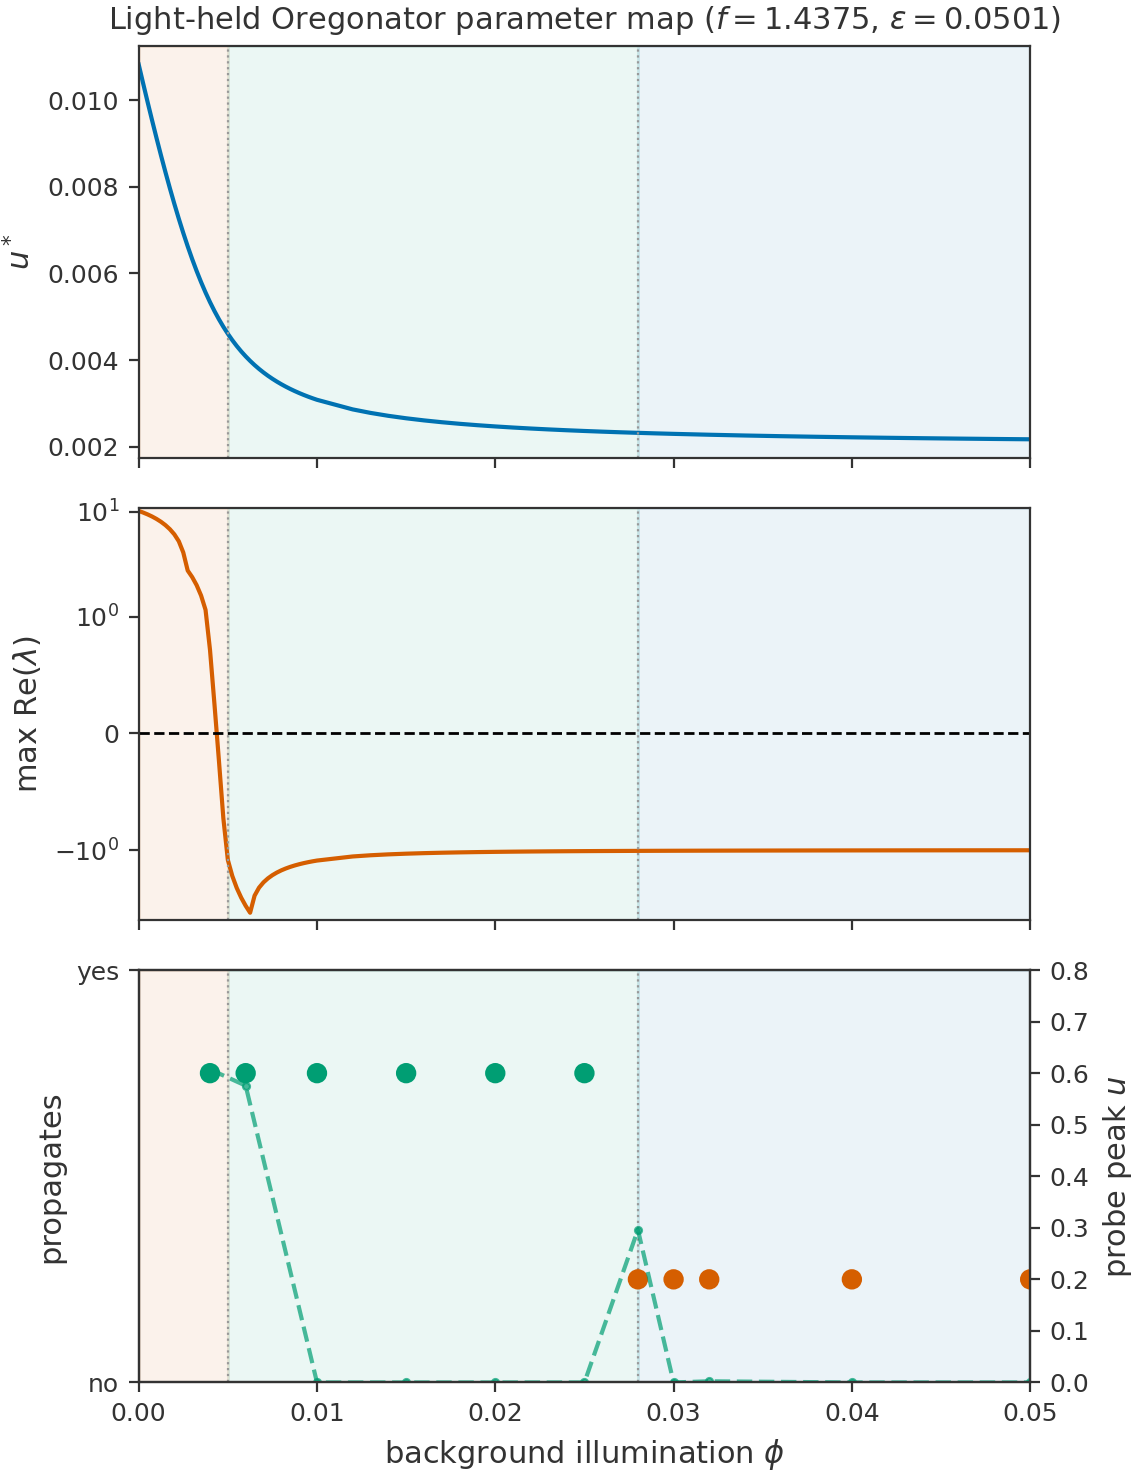
\includegraphics[width=0.85\textwidth]{../Analysis/figures/pub/pub_regime_map.png}}{%
[figure pending]}
\caption{Oregonator regime map in the $(\varepsilon, \phi)$ plane. The excitable propagation band lies between the oscillatory and attenuated regimes; the working point is marked near the centre of the band.}
\label{fig:meth_regime}
\end{figure}

\section{Numerical Solver and Verification}
\label{sec:meth_solver}

\subsection{Discretisation}
\label{sec:meth_discretisation}

The equations are discretised on a regular two-dimensional Cartesian grid with spacing $\Delta x = 1$ cell and time step $\Delta t = 0.05$ time units.
The diffusion term is discretised in divergence (flux) form, with face-averaged tensors and central differences, reducing to the standard five-point Laplacian when the tensor is isotropic.
No-flux walls are enforced at the flux level by zeroing fluxes on wall-adjacent faces.
The explicit diffusion stability constraint $D\,\Delta t / \Delta x^{2} \leq 1/4$ is satisfied at the working resolution.

The fast activator kinetics are stiff, so time integration uses first-order operator splitting with adaptive reaction subcycling.
Within each outer step the reaction substep $h$ is chosen from the analytic Jacobian: $h \leq 0.5 / \max(-\partial F/\partial u,\,0)$.
A relative-accuracy limit and an absolute step-size limiter prevent $u$ from being pushed below $-q/2$ complete the rule.
A NaN/Inf tripwire aborts any run in which a field leaves the finite range.

\subsection{Verification Cases}
\label{sec:meth_verification}

The solver was verified against canonical excitable-media phenomenology: target waves, head-on collision and annihilation, gap diffraction, and timing control.
Grid refinement at $\Delta x = 1$, $0.5$, $0.25$ and timestep refinement about $\Delta t = 0.05$ were applied to the plane-pulse speed.
The full convergence study is reported in \refSec{sec:res_verification}; the spatial deficit is carried openly as an explicit error bar wherever absolute speeds are quoted.

\section{Substrate Parameterisation}
\label{sec:meth_parameterisation}

Three physically distinct parameterisations are used.

\subsection{Wall Geometry}
\label{sec:meth_walls}

Walls are a boolean mask; masked cells are impermeable and no-flux conditions are enforced at adjacent faces.
They define input ports, channels, and junctions.

\subsection{Light-Suppression Field}
\label{sec:meth_light}

The field $\phi(x,y)$ enters through the term $(f v + \phi)(u-q)/(u+q)$ in \refeqn{eq:oregonator_u}; locally increasing $\phi$ raises the effective threshold and suppresses excitability.
A uniform background value sets the operating regime; spatial modulation defines rewritable channels and barriers.

\subsection{Anisotropic Diffusion Tensor}
\label{sec:meth_anisotropy}

The activator diffusivity is replaced by a symmetric positive-definite tensor field $\mathbf{D}(x,y)$, parameterised by eigenvalues $D_{\parallel} \geq D_{\perp} > 0$ and fibre direction $\theta(x,y)$.
Eikonal theory predicts the pulse speed along the fast axis exceeds that along the slow axis by $\sqrt{r}$, where $r = D_{\parallel}/D_{\perp}$ \cite{keener1991eikonal}.

\section{Black-Box Characterisation Protocol}
\label{sec:meth_protocol}

All experiments share a black-box protocol.
Inputs are applied at ports: small circular regions where the light field is temporarily reduced to emit pulses.
Outputs are recorded at probes: fixed locations storing the mean activator value $u(t)$ over a small mask.
The internal state away from ports and probes is not inspected for a measurement; every result is an input-output transfer function.

The dark-spot drive is a one-shot flash of darkness: a circular patch is dimmed from $\phi = 0.010$ to $\phi = 0.002$ for a calibrated duration.
Flashes of $T_{\mathrm{flash}} \leq 4$ time units emit exactly one full-amplitude pulse; the operating point used here is $T_{\mathrm{flash}} = 3.0$ time units.

\begin{figure}[htbp]
\centering
\IfFileExists{../Analysis/figures/pub/pub_flash_calibration.png}{%
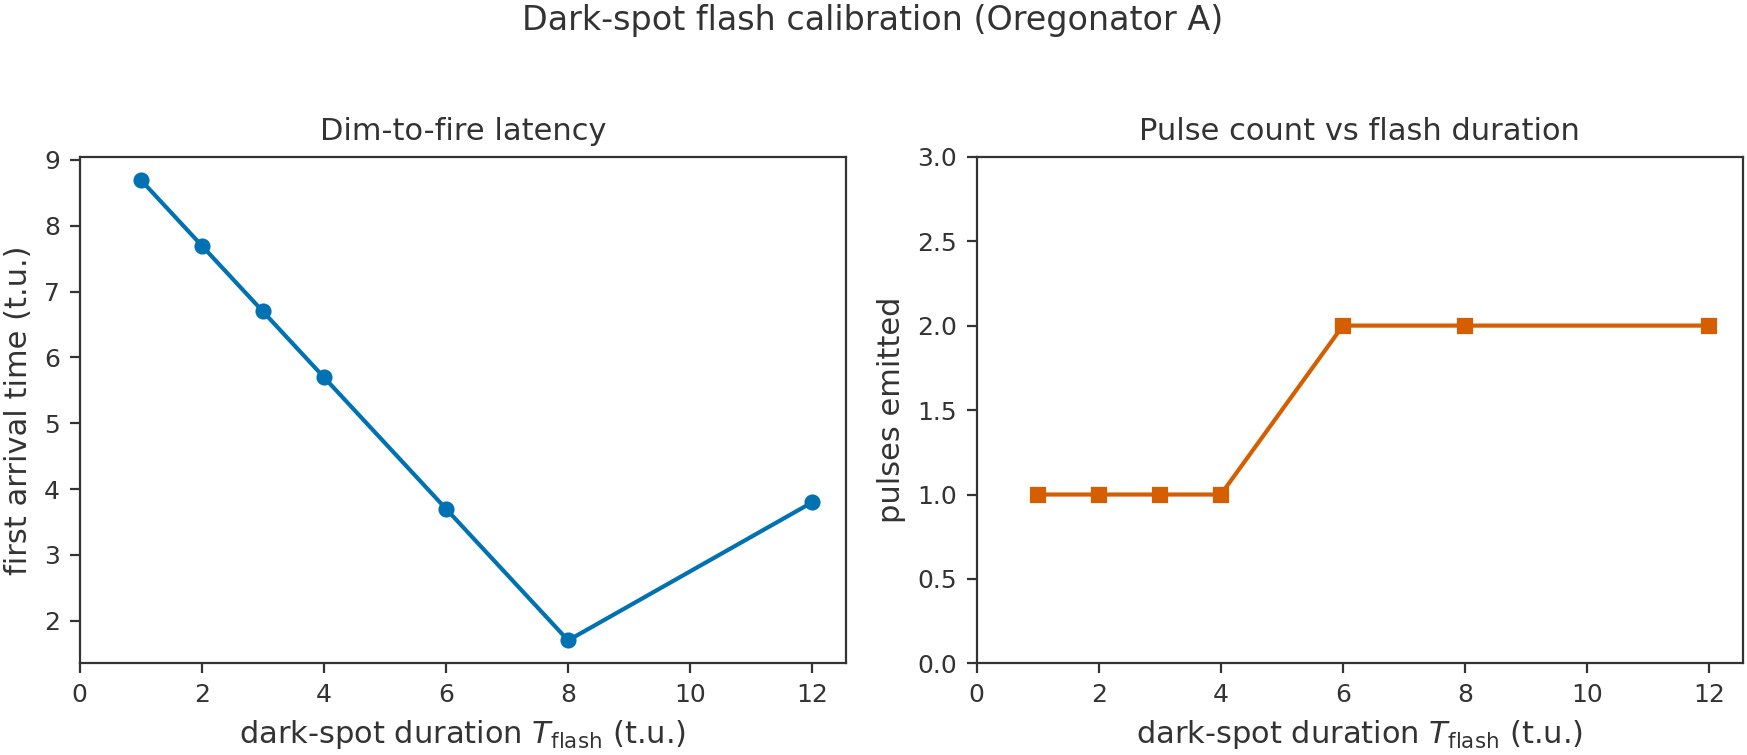
\includegraphics[width=0.85\textwidth]{../Analysis/figures/pub/pub_flash_calibration.png}}{%
[figure pending]}
\caption{Dark-spot flash calibration. Flash durations up to 4 time units emit a single pulse; longer flashes become sustained pacemakers. The operating point $T_{\mathrm{flash}} = 3.0$ time units is marked.}
\label{fig:meth_flash}
\end{figure}

Probe readouts are evaluated within defined time windows rather than over the whole record, because at an open junction a lone pulse diffracts into all connected branches and a whole-record readout would compute OR regardless of design intent.
The window is aligned to the expected collision outcome, isolating the annihilation event from the unconditional diffraction background.

\section{The Pore-Scale Experiments}
\label{sec:meth_experiments}

\subsection{Channel Pulse Transfer}
\label{sec:meth_exp_channel}

A straight channel of fixed width is cut between two walls, a single pulse is injected at the input port, and a far probe records the arrival.
Measured quantities: propagation speed, delay linearity, and transmission behaviour as width is swept.

\subsection{Frequency Response}
\label{sec:meth_exp_frequency}

A pulse train of prescribed frequency is injected and the probe records which pulses transmit.
Two forms: a two-pulse interval sweep locating the absolute refractory period, and a sustained-train measurement giving the maximum 1:1 following rate.

\subsection{Two-Input Inhibition}
\label{sec:meth_exp_logic}

Two input channels converge on a T-junction.
The four input combinations of a two-input truth table are applied; the probe record is converted into truth-table entries using the windowed readout.
Figures of merit: truth table, separation ratio, and inhibition window.

\subsection{Anisotropic Routing}
\label{sec:meth_exp_anisotropy}

In a uniform tensor field with anisotropy ratio $r$, a point stimulus is fired and the expanding pulse is tracked.
The $\sqrt{r}$ eikonal law provides a quantitative check, and a patch of anisotropic medium embedded in isotropic substrate measures orientation-dependent delay.

\section{Graph Simulator Construction}
\label{sec:meth_graph}

The measured transfer functions are translated into an event-driven graph simulator.
A node represents a pore or junction; an edge represents a throat.
Each edge carries a transit time $L/c$, where $L$ is the edge length in cells and $c$ is the measured pulse speed.
Each node carries a refractory time $\tau$, the interval after a pulse arrives during which the node ignores further pulses.
Each node also carries an inhibition window $w$: two pulses arriving at the same node within $w$ time units annihilate.
A routing table at each node decides which incoming edges feed which outgoing edges, encoding the junction topology.

The simulator processes pulses in order of arrival time.
When a pulse reaches a node, it is dropped if the node is refractory or if another pulse arrived within the inhibition window; otherwise it marks the node refractory and forwards copies to the allowed outgoing edges.
The simulator returns the arrival times and amplitudes at every probe.
It is fast enough to explore candidate networks in milliseconds, and its predictions are validated against PDE solutions in \refSec{sec:res_graph}.

\section{Three-Dimensional Extension}
\label{sec:meth_3d}

The graph simulator is dimensionless; the same nodes, edges, and rules apply in any dimension.
Extending the PDE solver to three dimensions requires a 7-point diffusion stencil, a 3D wall mask, and a 3D $\phi$ field.
The explicit stability limit becomes $D\,\Delta t / \Delta x^{2} \leq 1/6$.
Memory and compute grow as the cube of the linear domain size.

The practical blocker for full 3D pore networks is not the numerics but the light field: a projected 2D mask only controls the surface or a thin slab of a 3D bulk.
Without a known $\phi(x,y,z)$ in the interior, the local kinetics are uncontrolled.
The 3D results in \refSec{sec:res_3d} therefore use a thin-slab geometry and treat the extension as a boundary experiment rather than a validated network.


\chapter{Results and Discussion}
\label{chap:results}
% Chapter: Results and Discussion (porous reframe)

\section{Solver Verification}
\label{sec:res_verification}

Before any transfer function was trusted, the solver was verified by the method of manufactured solutions and by grid and timestep convergence studies.
\reffig{fig:res_verification} summarises the canonical test cases used to validate the solver against known excitable-media phenomenology.
\reffig{fig:res_mms} shows the measured error norms against grid spacing and time step.

\begin{figure}[htbp]
\centering
\IfFileExists{../Analysis/figures/pub/pub_verification.png}{%
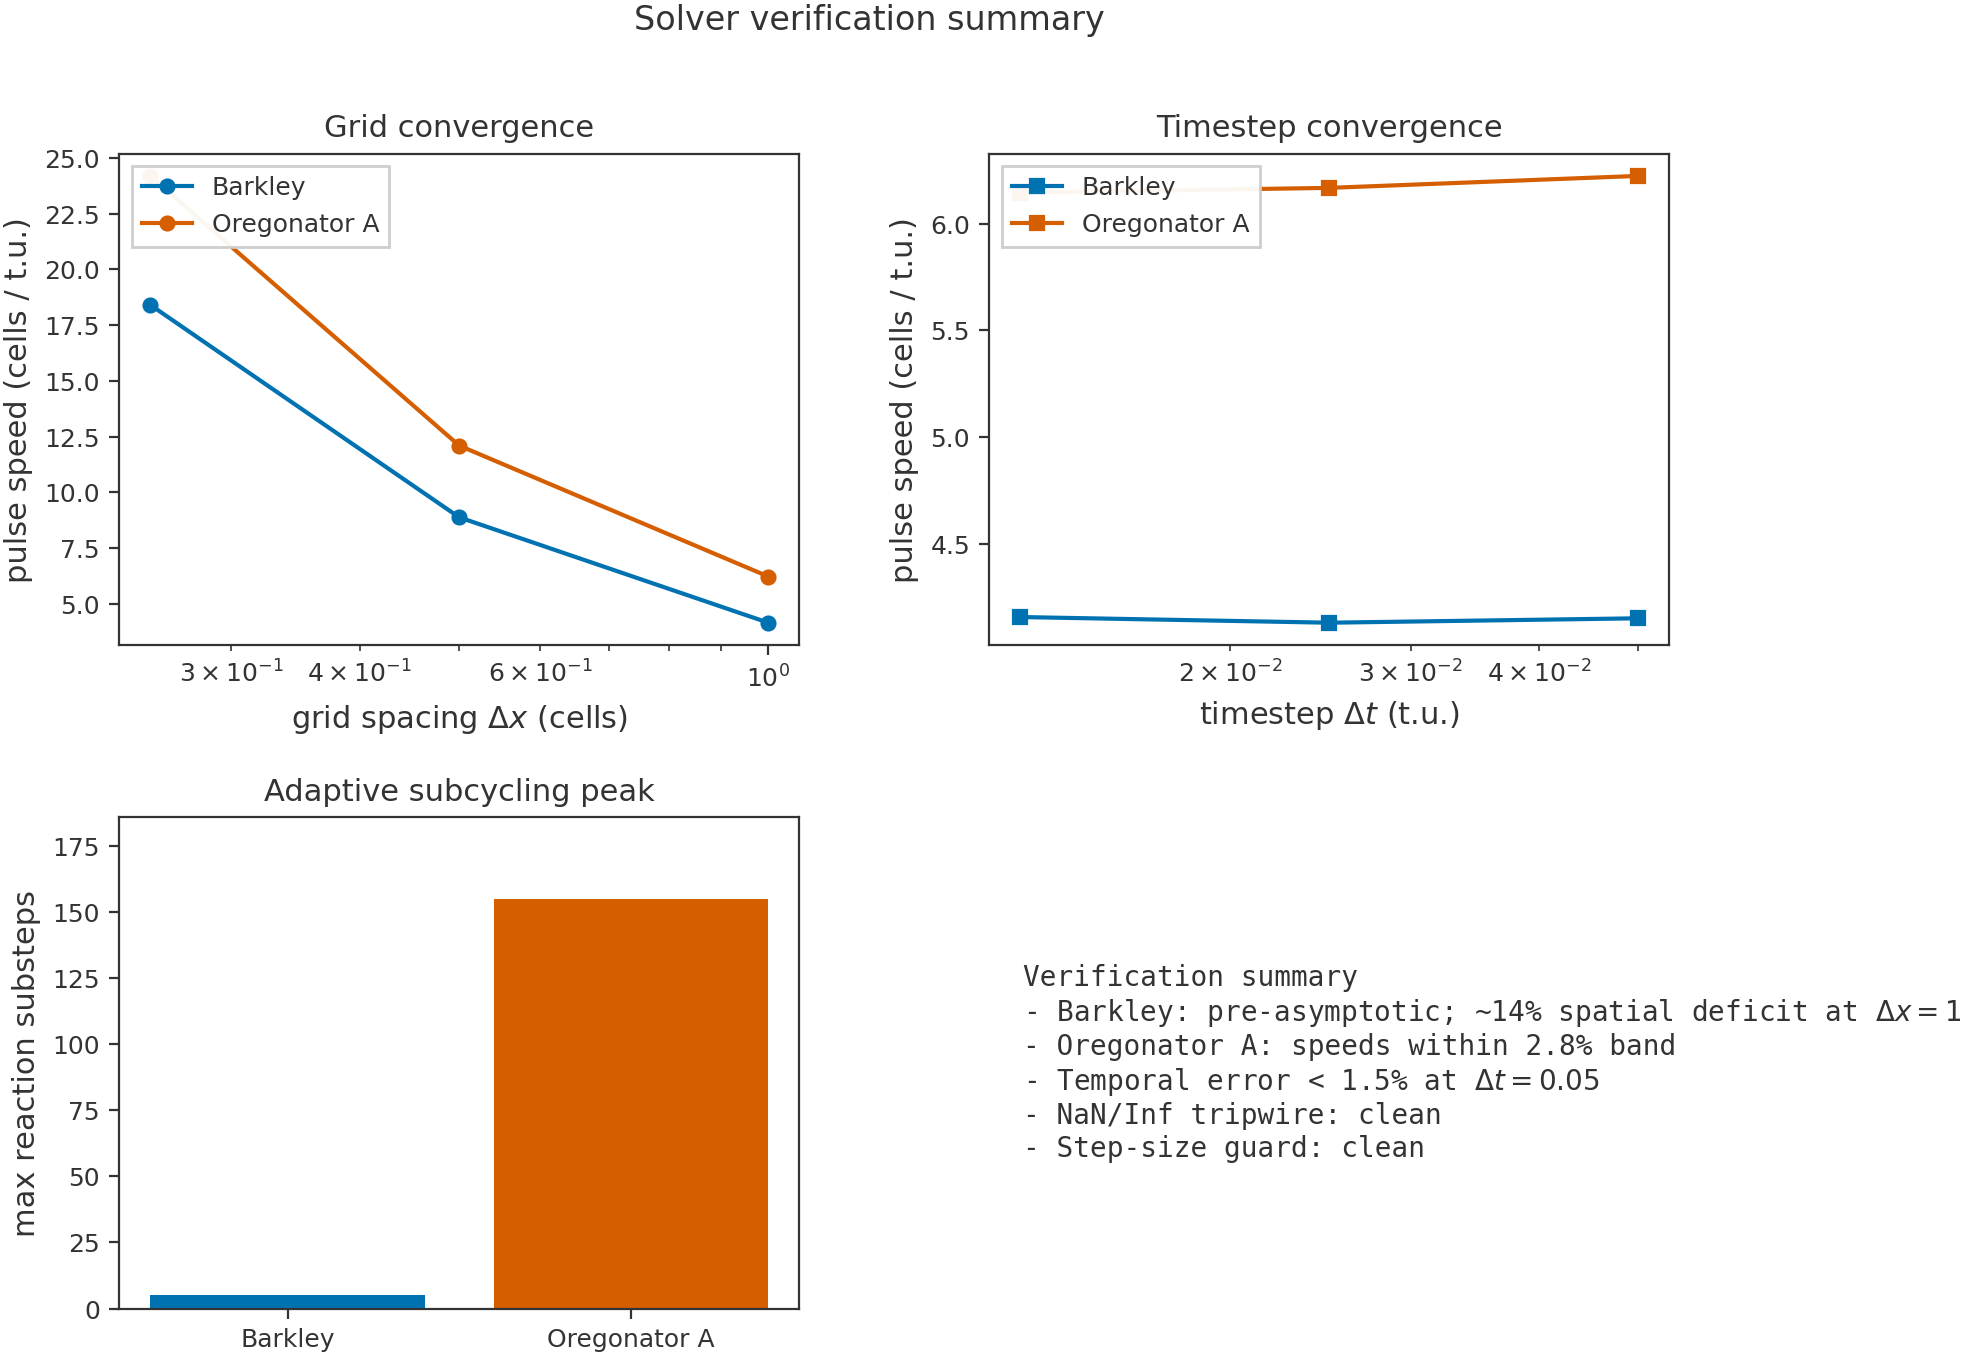
\includegraphics[width=0.95\textwidth]{../Analysis/figures/pub/pub_verification.png}}{%
[figure pending]}
\caption{Solver verification gallery: target waves, head-on collision and annihilation, gap diffraction, and timing control in the Oregonator model.}
\label{fig:res_verification}
\end{figure}
The observed spatial convergence orders at the finest refinement interval are $2.09$, $2.09$, and $1.99$ for Barkley isotropic, Barkley anisotropic, and Oregonator cases, against a design order of $2$.
The observed temporal orders are approximately $1.0$ across all cases, matching the first-order operator splitting.

Plane-pulse speed convergence is summarised in \reftab{tab:res_convergence}.
The Barkley sequence is pre-asymptotic, rising from $4.151$ cells per time unit at $\Delta x = 1$ to $4.603$ at $\Delta x = 0.25$; a Richardson extrapolation gives a continuum asymptote of approximately $4.82$, so the working resolution underestimates the Barkley speed by about $14\%$.
The Oregonator candidate-A speeds, $6.224$, $6.048$, and $6.049$, lie within a $2.8\%$ band, close to grid-converged at the working resolution.
All measurements reported below share the working resolution, so they are internally consistent as relative transfer-function measurements, and the absolute Barkley spatial deficit is stated as an explicit error bar.

\begin{figure}[htbp]
\centering
\IfFileExists{../Analysis/figures/pub/pub_mms_convergence.png}{%
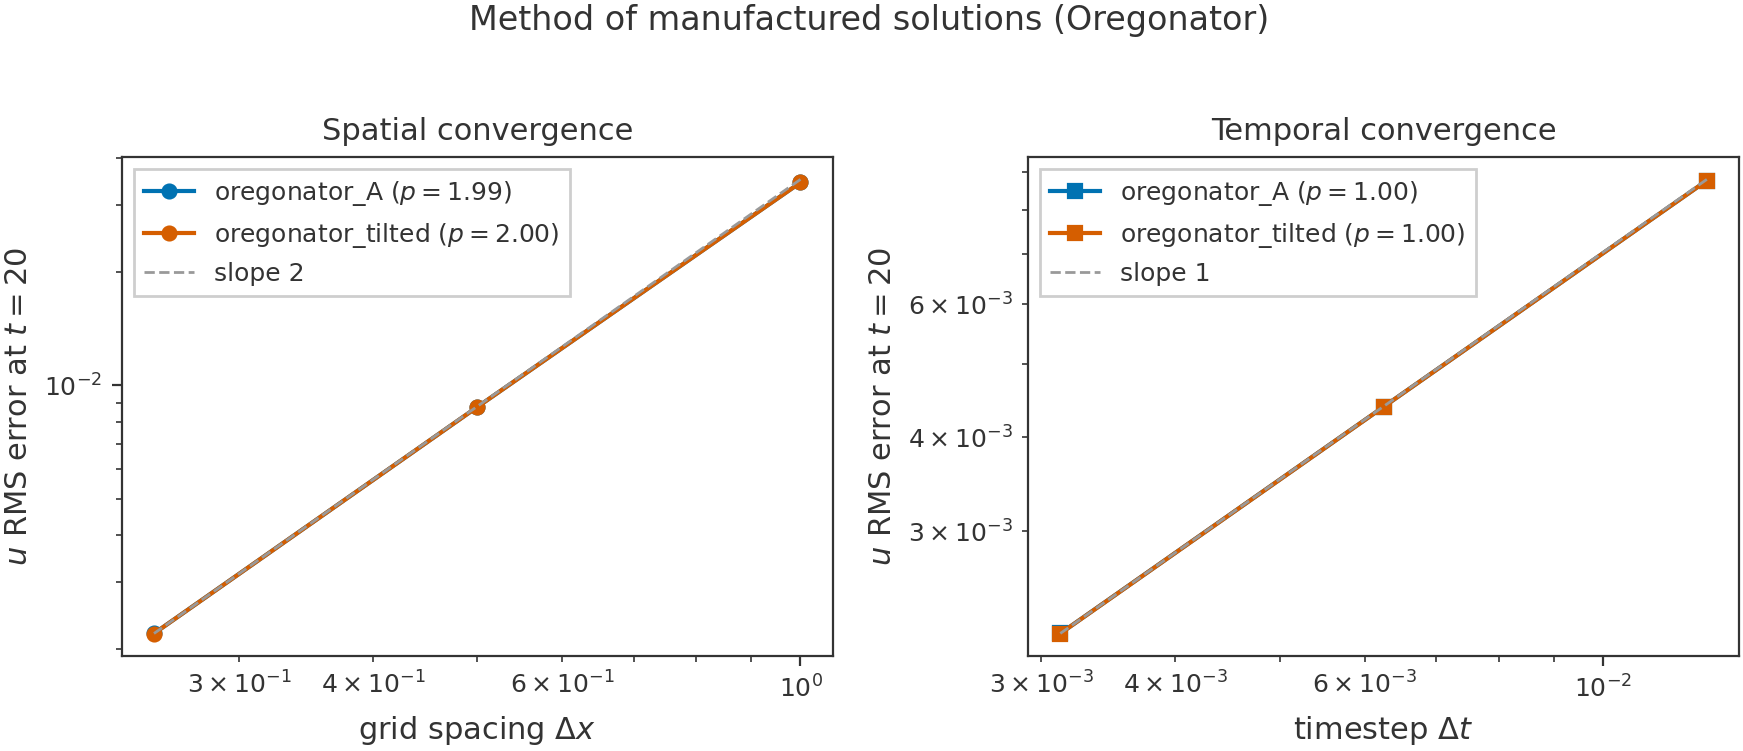
\includegraphics[width=0.9\textwidth]{../Analysis/figures/pub/pub_mms_convergence.png}}{%
[figure pending]}
\caption{Method of manufactured solutions: measured error norms against grid spacing and time step for Barkley isotropic, Barkley anisotropic, and Oregonator cases. Spatial orders are near $2$; temporal orders are near $1$.}
\label{fig:res_mms}
\end{figure}

\begin{table}[htbp]
\centering
\caption{Grid convergence of plane-pulse speed (cells per time unit) at $\Delta t = 0.05$.}
\label{tab:res_convergence}
\small
\begin{tabular}{@{}ccc@{}}
\toprule
$\Delta x$ (cells) & Barkley speed & Oregonator A speed \\
\midrule
1.00 & 4.151 & 6.224 \\
0.50 & 4.439 & 6.048 \\
0.25 & 4.603 & 6.049 \\
\midrule
Richardson asymptote & $\approx 4.82$ & n/a \\
\bottomrule
\end{tabular}
\end{table}

\section{Channel Pulse Transfer}
\label{sec:res_channel}

The wire operator was measured in a straight channel of width $W$.
A circular dark spot of radius 6 cells at the channel entrance emits a single pulse.
The free-medium dark-spot speed is $6.46$ cells per time unit and the channel speed is $6.46$--$6.47$ cells per time unit for every width from $W = 60$ down to $W = 1$.
The pulse transmits with undiminished amplitude, and no geometric wave block was observed.

The physics is that a planar front has zero curvature, so the eikonal curvature correction to its speed vanishes \cite{keener1991eikonal}.
The no-flux walls impose a zero normal derivative that a planar front already satisfies, so propagation in the channel is equivalent to a one-dimensional cable.
A straight channel is therefore a near-perfect wire whose speed and amplitude are set by the kinetics alone; width offers no computational advantage.
Structure that computes must come from junctions, curvature, or property fields.

\begin{figure}[htbp]
\centering
\IfFileExists{../Analysis/figures/pub/pub_channel_transfer_darkspot.png}{%
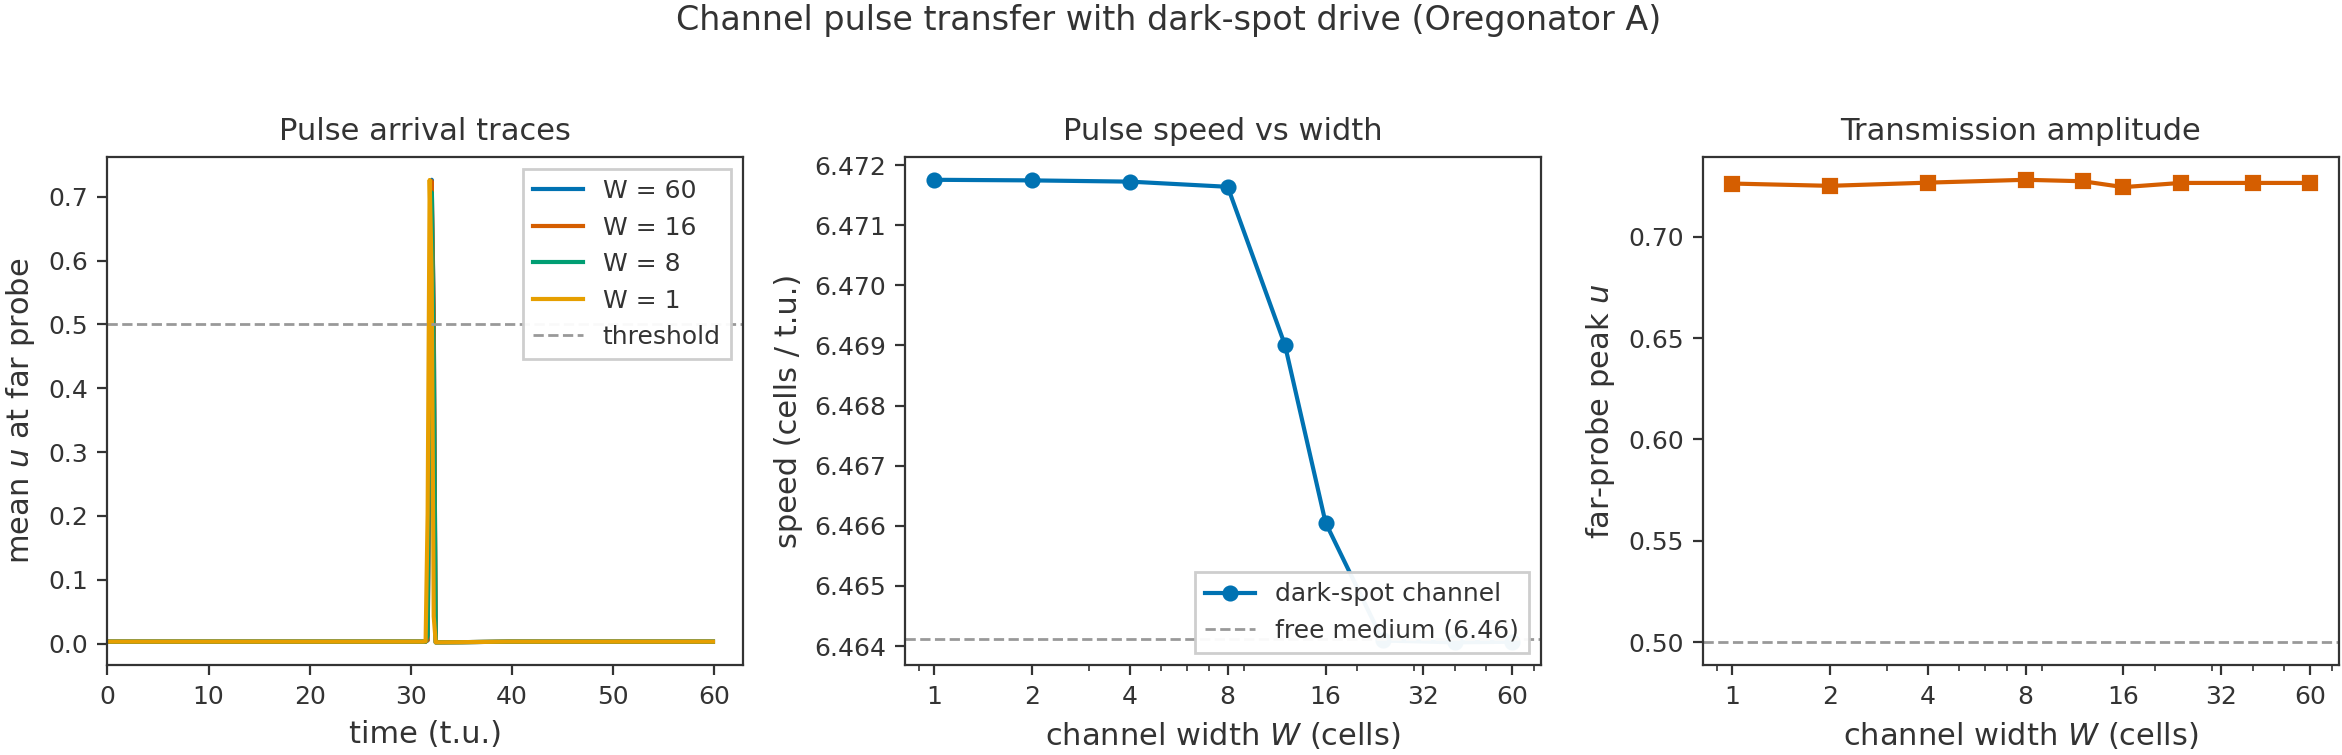
\includegraphics[width=0.9\textwidth]{../Analysis/figures/pub/pub_channel_transfer_darkspot.png}}{%
[figure pending]}
\caption{Channel pulse transfer with the dark-spot drive. A single pulse travels at the free-medium speed independent of channel width, confirming that a straight throat acts as a near-perfect wire.}
\label{fig:res_channel}
\end{figure}

\section{Frequency Response}
\label{sec:res_frequency}

The bandwidth of the wire is set by refractoriness.
The two-pulse measurement locates the absolute refractory period at $3.0$ time units for the Oregonator at candidate A.
Sustained pulse trains give the transmission curve of \reffig{fig:res_frequency}.
At low frequency the output follows the input one-to-one; the maximum 1:1 following rate is $0.167$ per time unit.
Above this rate the curve leaves unit slope and develops a staircase of dropped pulses.

The maximum 1:1 rate lies below the naive inverse of the refractory period because the dark-spot encoder itself imposes a minimum period: a flash of $3.0$ time units cannot be repeated faster than about $6.0$ time units without merging into one long pacemaker flash.
For single-event computation this constraint is irrelevant.

\begin{figure}[htbp]
\centering
\IfFileExists{../Analysis/figures/pub/pub_frequency_response_darkspot.png}{%
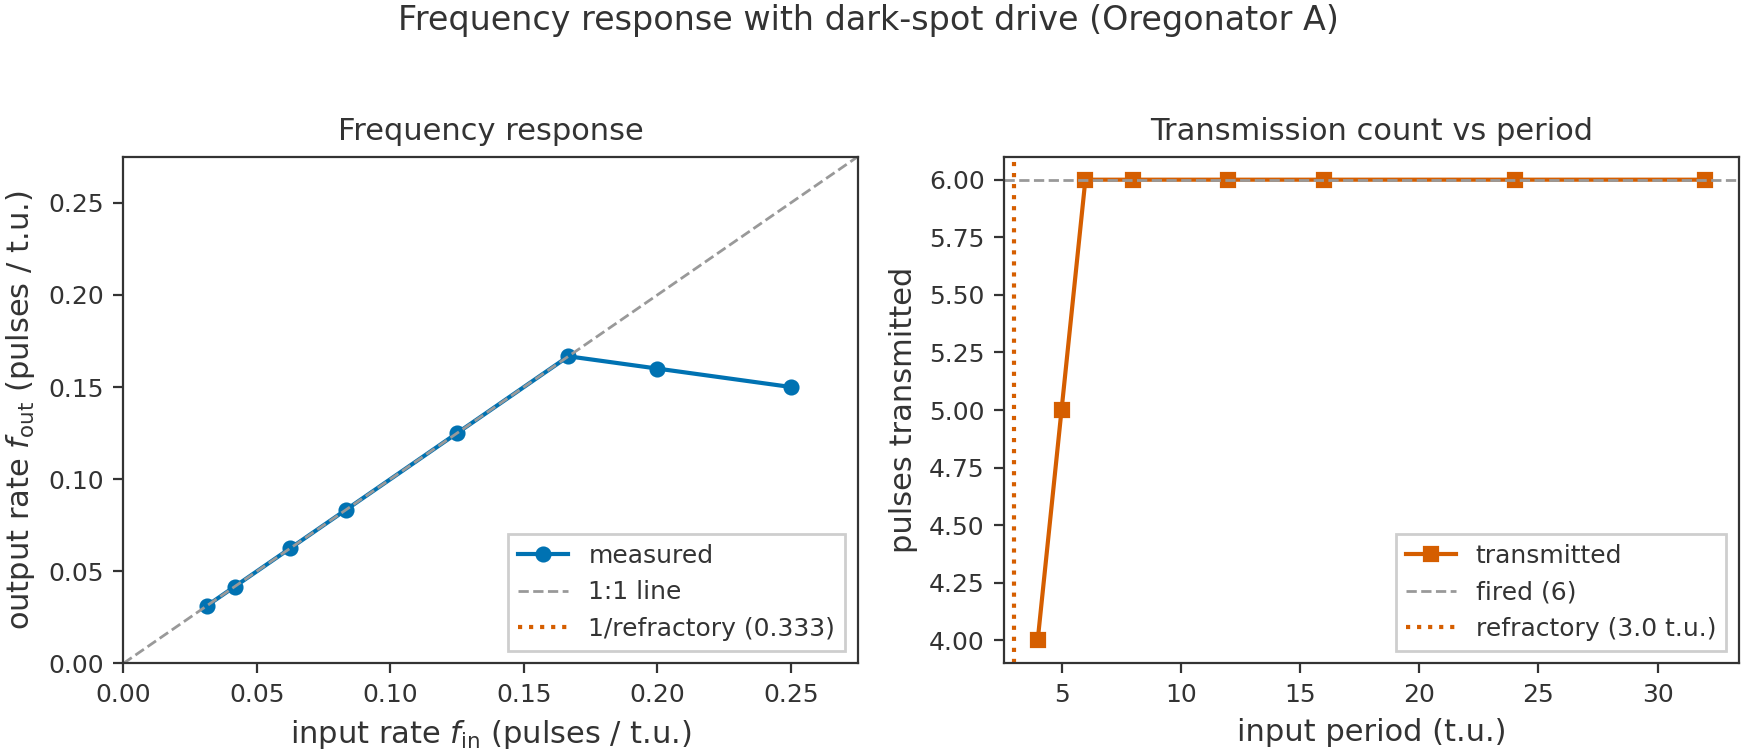
\includegraphics[width=0.85\textwidth]{../Analysis/figures/pub/pub_frequency_response_darkspot.png}}{%
[figure pending]}
\caption{Frequency response with the dark-spot drive (Oregonator A). The absolute refractory period is $3.0$ time units; the maximum 1:1 following rate is $0.167$ per time unit.}
\label{fig:res_frequency}
\end{figure}

\section{Two-Input Inhibition}
\label{sec:res_logic}

At a T-junction, the naive whole-record readout computes OR because a lone pulse diffracts into all connected branches.
With the windowed readout of \refSec{sec:meth_protocol}, the junction implements a genuine inhibition gate.
\reftab{tab:res_logic} gives the truth table for A AND (NOT B): the output probe fires when A fires alone, and is suppressed when B fires alone or when both fire.

\begin{table}[htbp]
\centering
\caption{PDE truth table for the A AND (NOT B) inhibition gate, measured in a T-junction with windowed readout.}
\label{tab:res_logic}
\small
\begin{tabular}{cccc}
\toprule
Pattern & Output peak & Output fires? \\
\midrule
00 & 0.000 & no \\
01 (B only) & 0.003 & no \\
10 (A only) & 0.706 & yes \\
11 (A+B) & 0.003 & no \\
\bottomrule
\end{tabular}
\end{table}

The separation ratio between the true output (0.706) and the strongest false output (0.003) is over $200\times$.
This inhibition operator is one of the primitives used in the graph simulator.

\begin{figure}[htbp]
\centering
\IfFileExists{../Analysis/figures/pub/pub_tjunction_logic_darkspot.png}{%
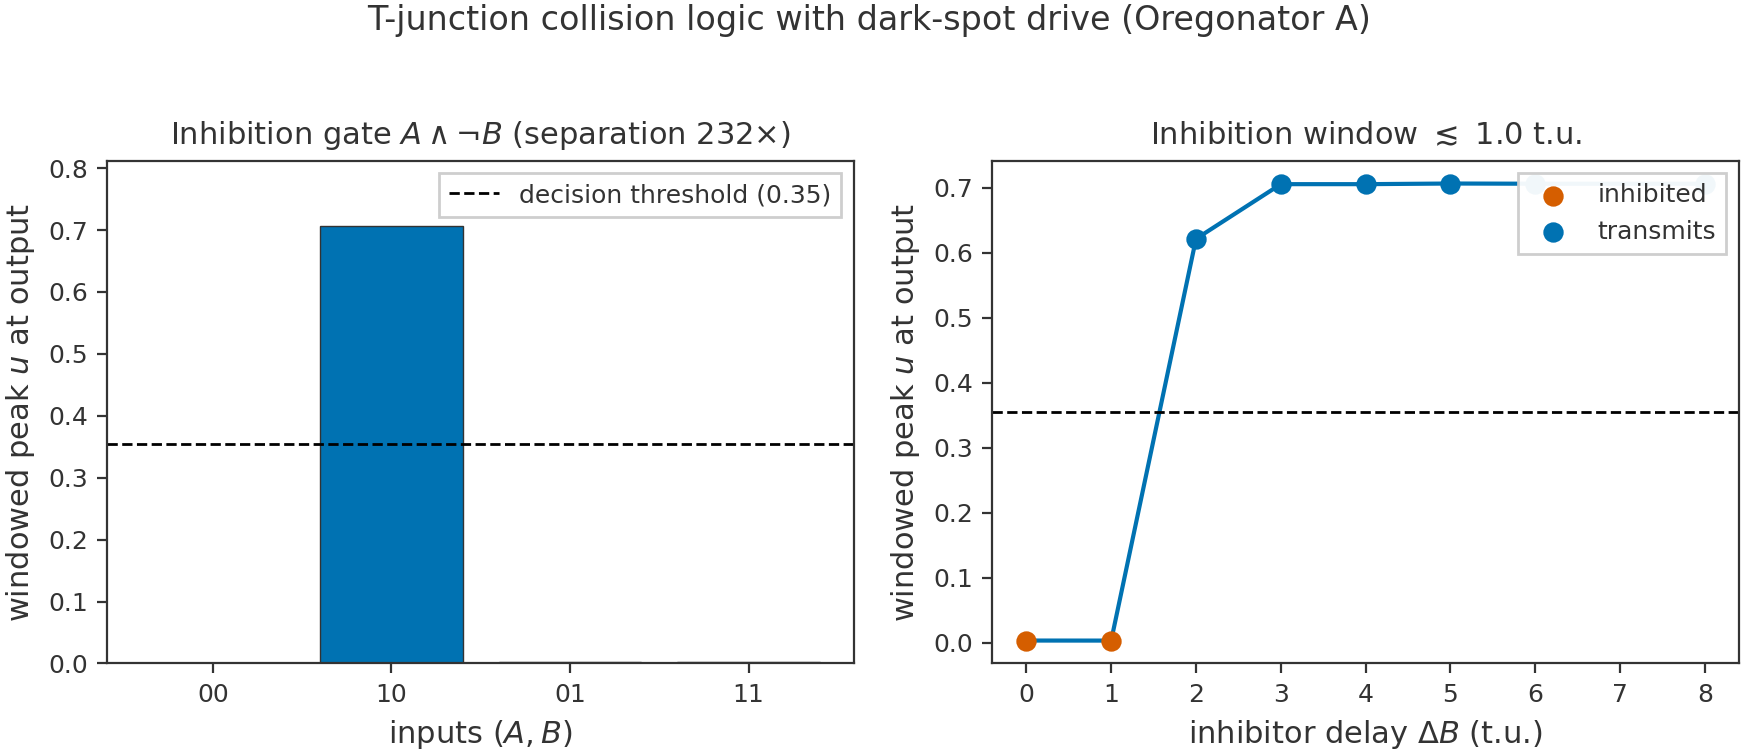
\includegraphics[width=0.9\textwidth]{../Analysis/figures/pub/pub_tjunction_logic_darkspot.png}}{%
[figure pending]}
\caption{T-junction inhibition gate with windowed readout. A alone reaches the output; B alone and A+B are suppressed, giving A AND (NOT B).}
\label{fig:res_logic}
\end{figure}

\section{Anisotropic Routing}
\label{sec:res_anisotropy}

A uniform anisotropic diffusion tensor with ratio $r = D_{\parallel}/D_{\perp}$ produces elliptical wave fronts whose fast-to-slow speed ratio is $\sqrt{r}$, confirming the eikonal prediction \cite{keener1991eikonal}.
A patch of anisotropic medium embedded in an isotropic substrate introduces direction-dependent delays.
This gives a continuous routing knob that neither walls nor light provide.

\begin{figure}[htbp]
\centering
\IfFileExists{../Analysis/figures/pub/pub_anisotropic_routing.png}{%
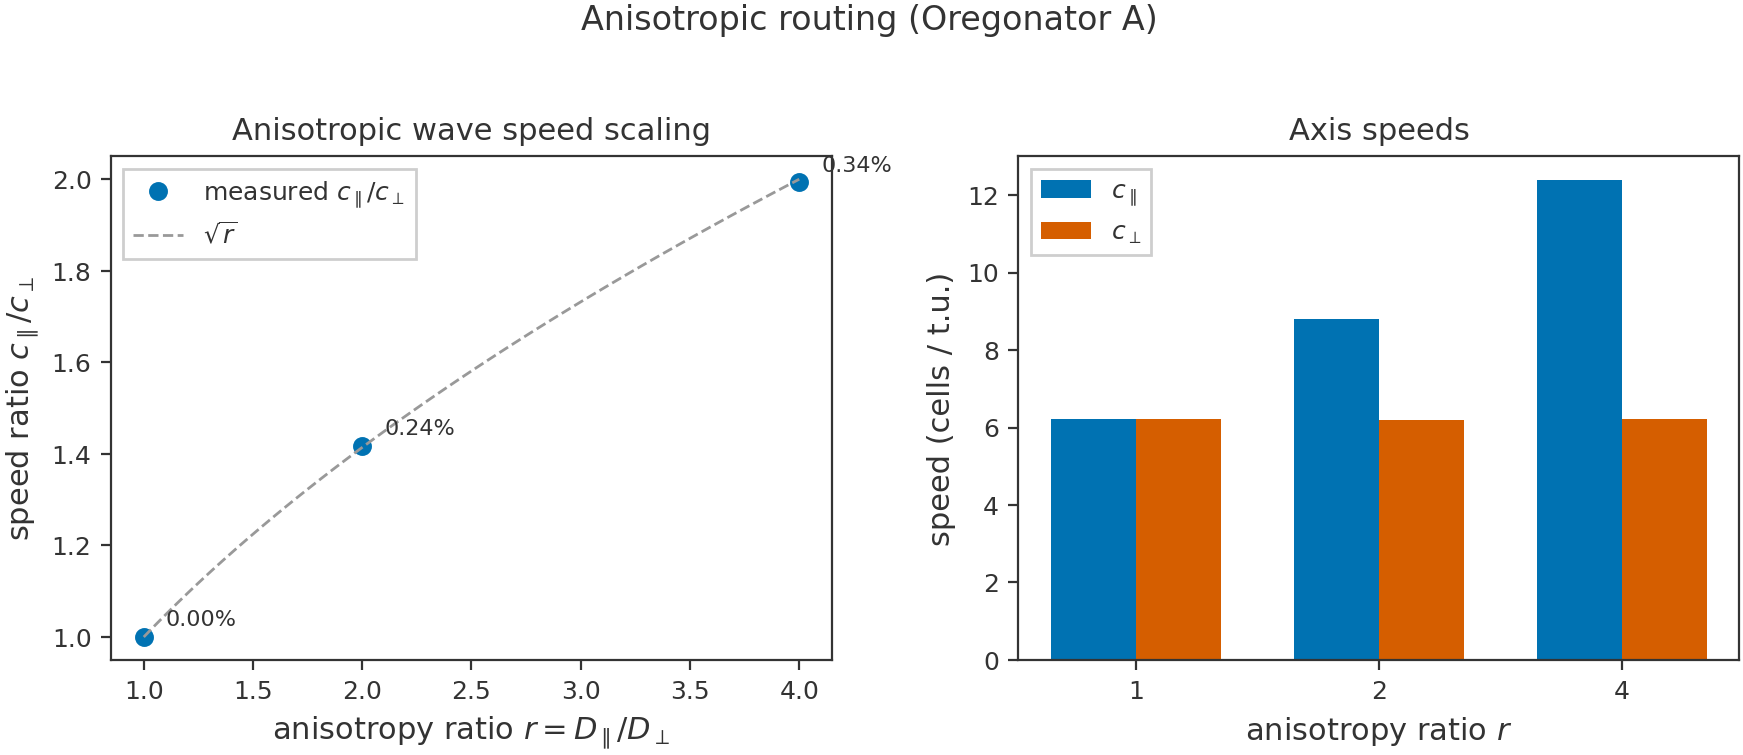
\includegraphics[width=0.9\textwidth]{../Analysis/figures/pub/pub_anisotropic_routing.png}}{%
[figure pending]}
\caption{Anisotropic routing. Elliptical wave fronts in a uniform tilted tensor field follow the eikonal $\sqrt{r}$ speed law, and an embedded anisotropic patch produces orientation-dependent delays.}
\label{fig:res_anisotropy}
\end{figure}

\section{Graph-Simulator Validation}
\label{sec:res_graph}

The measured operators were translated into the event-driven graph simulator of \refSec{sec:meth_graph}.
Three circuits were validated against full PDE solutions.

\subsection{Inhibition Gate}
\label{sec:res_graph_andnot}

The T-junction inhibition gate was modelled as a graph with nodes A, B, J, OUT and edges A$\rightarrow$J, B$\rightarrow$J, J$\rightarrow$OUT.
The routing table at J sends A to OUT and B nowhere.
\reftab{tab:res_graph_andnot} compares the graph prediction with the PDE measurement.

\begin{table}[htbp]
\centering
\caption{Graph simulator versus PDE for the A AND (NOT B) gate.}
\label{tab:res_graph_andnot}
\small
\begin{tabular}{ccccc}
\toprule
Pattern & Graph output & Graph arrival (t.u.) & PDE output peak & Match? \\
\midrule
00 & none & none & 0.000 & yes \\
01 & none & none & 0.003 & yes \\
10 & fires & 31.9 & 0.706 & yes \\
11 & none & none & 0.003 & yes \\
\bottomrule
\end{tabular}
\end{table}

The graph simulator captures the inhibition operator once the junction routing is encoded.

\subsection{Priority Router}
\label{sec:res_graph_router}

A 2-to-1 priority router was built from the same primitives: two input arms of different lengths merge into one output stem.
Arm A is shorter, so it reaches the junction first and makes it refractory; a coincident B pulse is blocked.
\reftab{tab:res_graph_router} compares graph and PDE predictions.

\begin{table}[htbp]
\centering
\caption{Graph simulator versus PDE for the 2-to-1 priority router.}
\label{tab:res_graph_router}
\small
\begin{tabular}{lccc}
\toprule
Pattern & Graph output & PDE output & Winner \\
\midrule
00 & none & none & none \\
01 (B only) & 1 pulse & 1 pulse & B \\
10 (A only) & 1 pulse & 1 pulse & A \\
11 (A+B) & 1 pulse & 1 pulse & A (shorter path) \\
\bottomrule
\end{tabular}
\end{table}

The graph simulator predicts the router before the PDE is run.

\subsection{Shared-Control Multi-Junction Gate}
\label{sec:res_graph_multi}

A shared-control gate was built in which one control input A can block two independent data paths B1 and B2.
The graph uses nodes A, B1, B2, J1, J2, O1, O2 with timing chosen so that A reaches each junction before the corresponding data pulse.
\reftab{tab:res_graph_multi} gives the graph truth table; it is correct for all eight input patterns.

\begin{table}[htbp]
\centering
\caption{Graph-simulator truth table for the shared-control gate.}
\label{tab:res_graph_multi}
\small
\begin{tabular}{ccc|cc}
\toprule
A & B1 & B2 & O1 fires? & O2 fires? \\
\midrule
0 & 0 & 0 & no & no \\
0 & 1 & 0 & yes & no \\
0 & 0 & 1 & no & yes \\
0 & 1 & 1 & yes & yes \\
1 & 0 & 0 & no & no \\
1 & 1 & 0 & no & no \\
1 & 0 & 1 & no & no \\
1 & 1 & 1 & no & no \\
\bottomrule
\end{tabular}
\end{table}

The PDE validation shows clean A-blocking for individual data pulses: O1 separation is $182\times$ and O2 separation is $192\times$.
However, pattern $011$ (both data pulses active, control absent) fails because B1 reaches J1 first, enters the shared horizontal control channel, and blocks J2 before B2 arrives.
This is a network-level crosstalk not captured by single-junction primitives.
It shows that the graph simulator must be calibrated per junction shape and that shared channels can introduce unmodelled coupling.

\begin{figure}[htbp]
\centering
\IfFileExists{../Analysis/figures/rd_multi_gate_pde_snapshots.png}{%
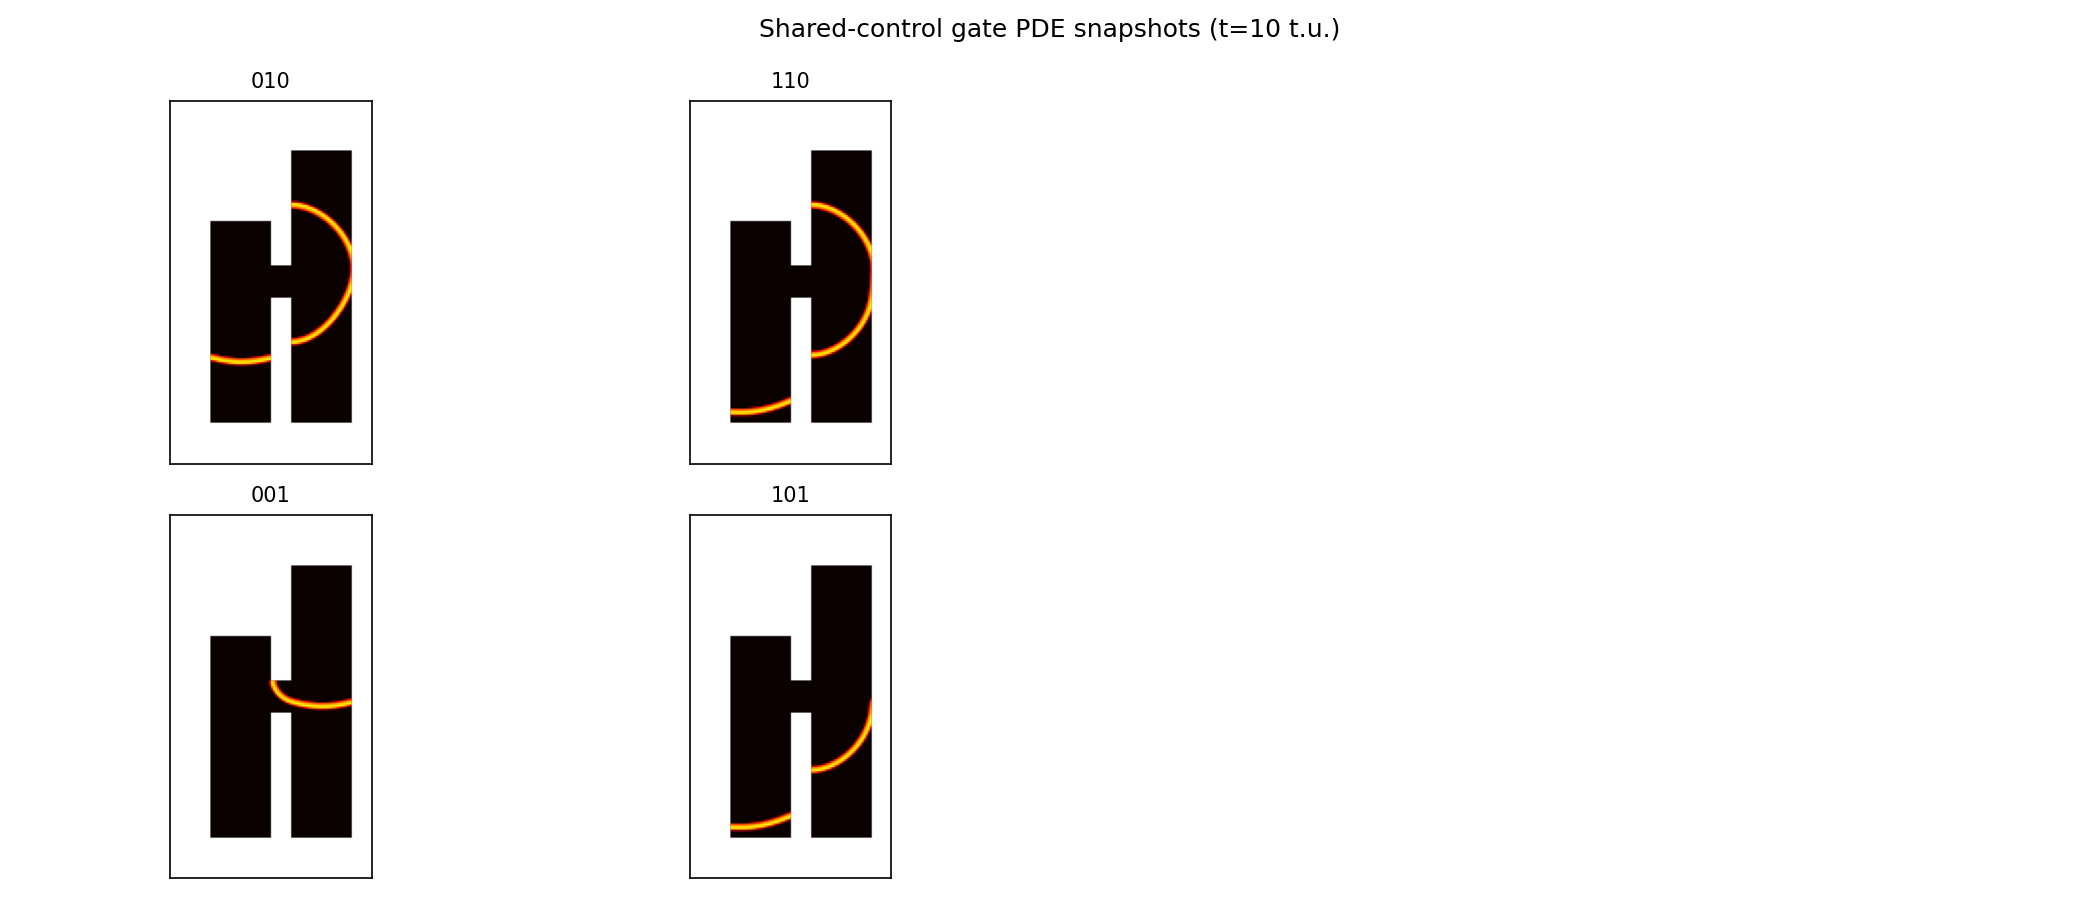
\includegraphics[width=0.95\textwidth]{../Analysis/figures/rd_multi_gate_pde_snapshots.png}}{%
[figure pending]}
\caption{Shared-control multi-junction gate. A single control pulse blocks both data paths, but pattern $011$ produces crosstalk when B1 enters the shared control channel and blocks J2 before B2 arrives.}
\label{fig:res_graph_multi}
\end{figure}

\section{Geometry-Dependent Failure of Collision XOR}
\label{sec:res_xor}

A symmetric Y-junction with a chamber was designed to implement collision XOR: a pulse on either input arm should reach the output, but two coincident pulses should annihilate and leave the output silent.
The graph model predicts this behaviour, but the PDE shows a leak.
\reftab{tab:res_xor} gives the result for a chamber radius $R = 25$ cells.

\begin{table}[htbp]
\centering
\caption{Collision-XOR prediction versus PDE in a chambered Y-junction.}
\label{tab:res_xor}
\small
\begin{tabular}{lcc}
\toprule
Pattern & Graph prediction & PDE (chamber $R = 25$) \\
\midrule
01 / 10 & output fires & output fires \\
11 & no output & output still fires \\
\bottomrule
\end{tabular}
\end{table}

The leak occurs because extended channel fronts collide but the excitation curves around the annihilation point and re-ignites the output stem.
Pattern $11$ still triggers crossings in the output arms, so the chamber geometry does not achieve clean collision XOR.
This confirms that inhibition rules are geometry-dependent: the graph model must be PDE-calibrated per junction shape, not assumed universal.

\begin{figure}[htbp]
\centering
\IfFileExists{../Analysis/figures/rd_spot_xor_protocol.png}{%
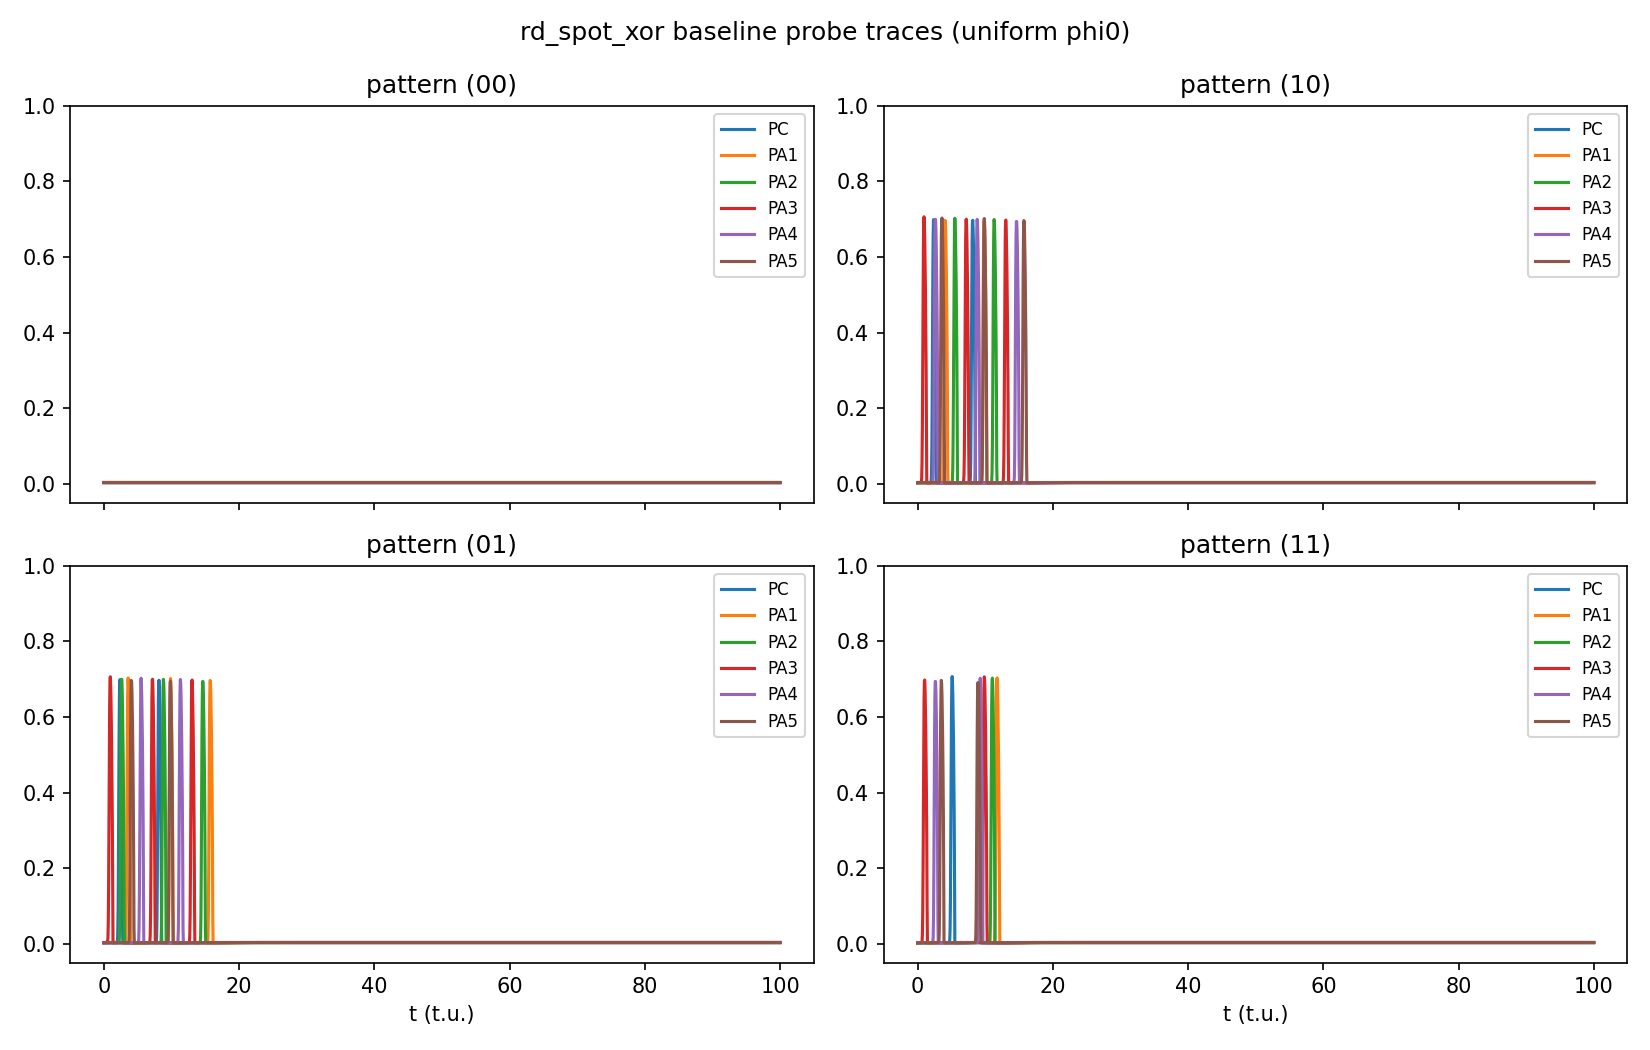
\includegraphics[width=0.95\textwidth]{../Analysis/figures/rd_spot_xor_protocol.png}}{%
[figure pending]}
\caption{Collision-XOR baseline in a chambered Y-junction. Lone input pulses reach the output, but the coincident-pulse case leaks because the collision re-ignites the output stem.}
\label{fig:res_xor}
\end{figure}

\section{Three-Dimensional Inhibition Gate}
\label{sec:res_3d}

The graph simulator is dimensionless, so the same rules apply in three dimensions.
To test whether the 2D operators transfer, a 3D T-junction inhibition gate was simulated in a $64 \times 48 \times 48$ domain.
The original geometry was a `+' intersection in which the vertical B channel had a downward outlet; this allowed B alone to reach the output, giving only a $2.5\times$ separation.
After closing the B outlet arm and scaling the arm lengths, the gate was recognised cleanly.
\reftab{tab:res_3d} gives the corrected 3D truth table.

\begin{table}[htbp]
\centering
\caption{Corrected 3D T-junction inhibition gate.}
\label{tab:res_3d}
\small
\begin{tabular}{ccc}
\toprule
inputs & window peak & comment \\
\midrule
00 & 0.003 & quiet \\
10 (A only) & 0.713 & A passes \\
01 (B only) & 0.042 & suppressed leakage \\
11 (A+B) & 0.042 & suppressed leakage \\
\bottomrule
\end{tabular}
\end{table}

The separation ratio is $16.8\times$ and A alone arrives at the probe at $8.25$ time units.
The 3D channel pulse speed is $6.62$ cells per time unit, close to the 2D value of $6.46$.
This shows that the micro-scale operators do transfer to a thin-slab 3D geometry once the junction shape is controlled.
A full 3D multi-gate network remains future work.

\begin{figure}[htbp]
\centering
\IfFileExists{../Analysis/figures/rd_3d_transfer_logic_snapshots.png}{%
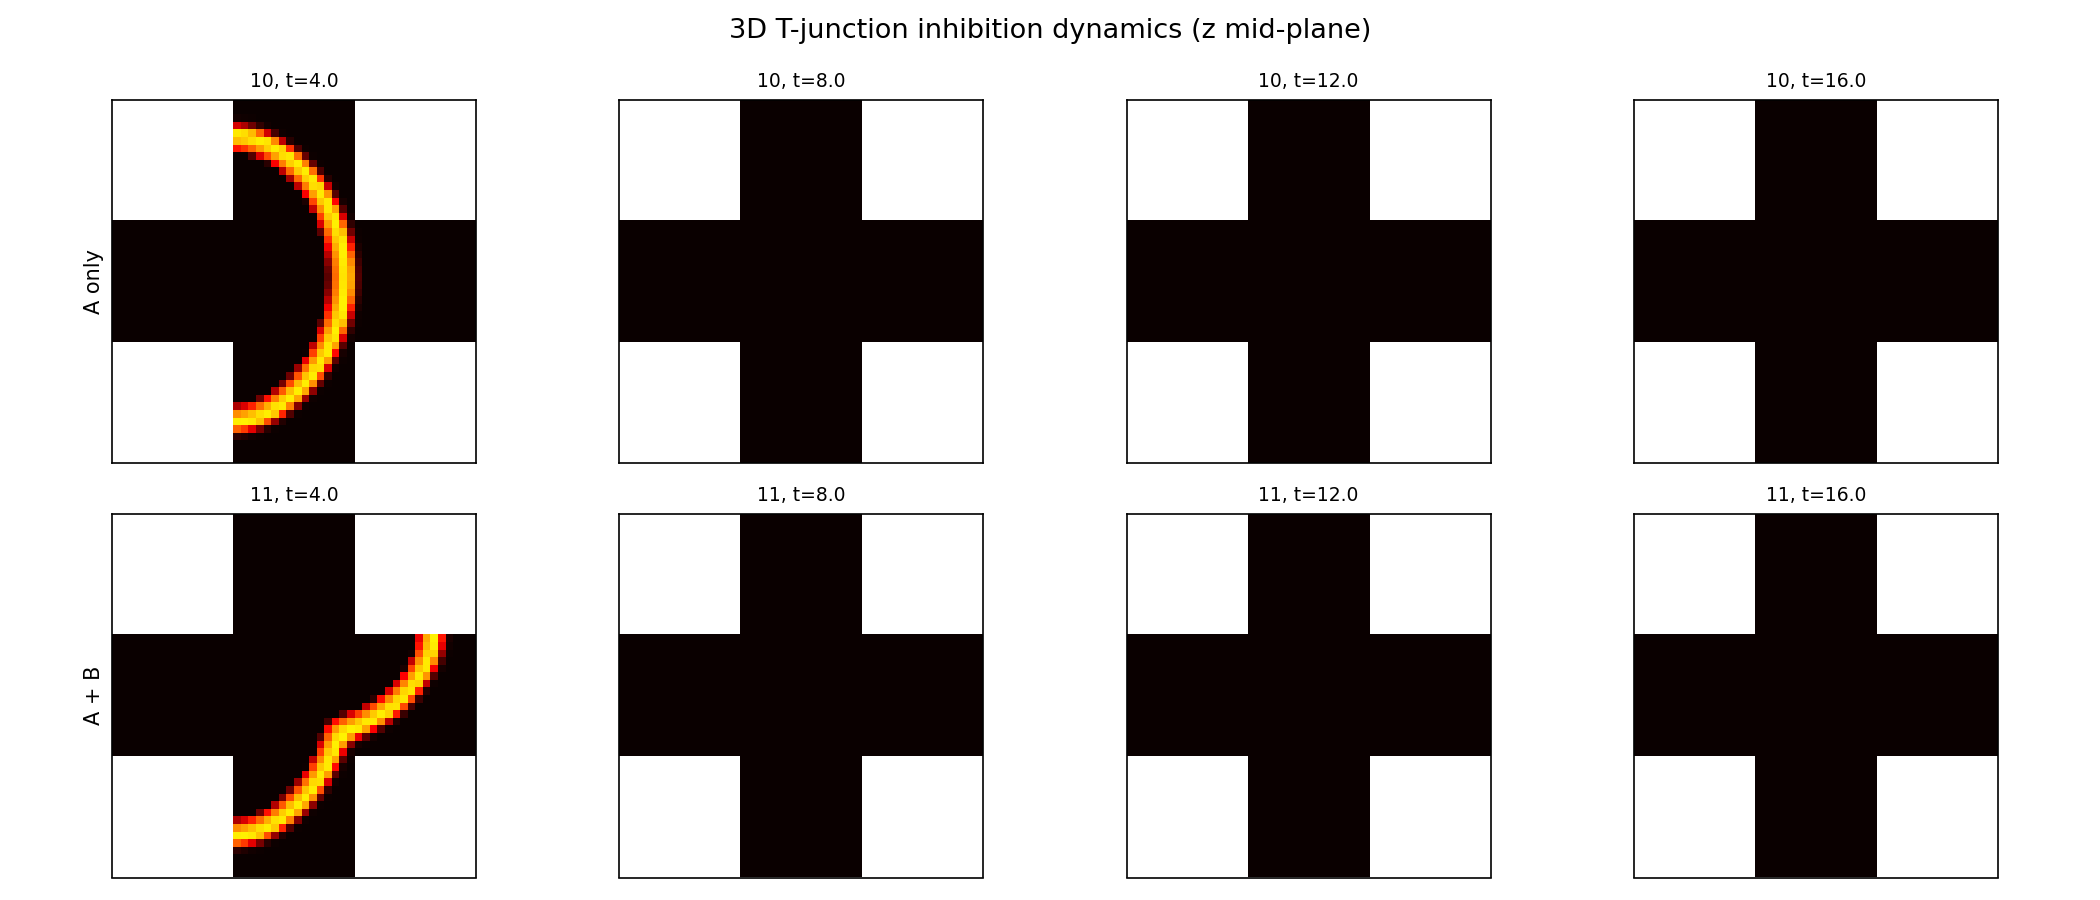
\includegraphics[width=0.95\textwidth]{../Analysis/figures/rd_3d_transfer_logic_snapshots.png}}{%
[figure pending]}
\caption{Three-dimensional T-junction inhibition gate. A alone reaches the output; B alone and A+B are suppressed after closing the B outlet arm and scaling the geometry.}
\label{fig:res_3d}
\end{figure}

\section{One-Way Diode Pilot}
\label{sec:res_diode}

A one-way pulse diode was tested in three forms: an asymmetric wall geometry (gradual taper on one side, abrupt step on the other), a straight channel with an asymmetric $\phi$ barrier, and a hybrid of the two.
\reftab{tab:res_diode} summarises the results.

\begin{table}[htbp]
\centering
\caption{One-way diode pilot results.}
\label{tab:res_diode}
\small
\begin{tabular}{lcccc}
\toprule
mode & forward peak & reverse peak & extinction ratio & diode works? \\
\midrule
geometry & 0.724 & 0.517 & 1.4 & no \\
light & 0.680 & 0.680 & 1.0 & no \\
hybrid & 0.724 & 0.517 & 1.4 & no \\
\bottomrule
\end{tabular}
\end{table}

The asymmetric wall geometry gives only a $1.4\times$ forward-to-reverse ratio, and the reverse pulse still crosses threshold.
The light-only barrier is symmetric because the static $\phi$ field spans both directions equally.
A simple asymmetric taper or static light barrier is therefore insufficient for robust rectification in the present parameter regime.
The diode is left as an open problem; candidate fixes include angled branches, absorbing side chambers, or timed refractory structures.

\begin{figure}[htbp]
\centering
\IfFileExists{../Analysis/figures/rd_diode_pilot_series.png}{%
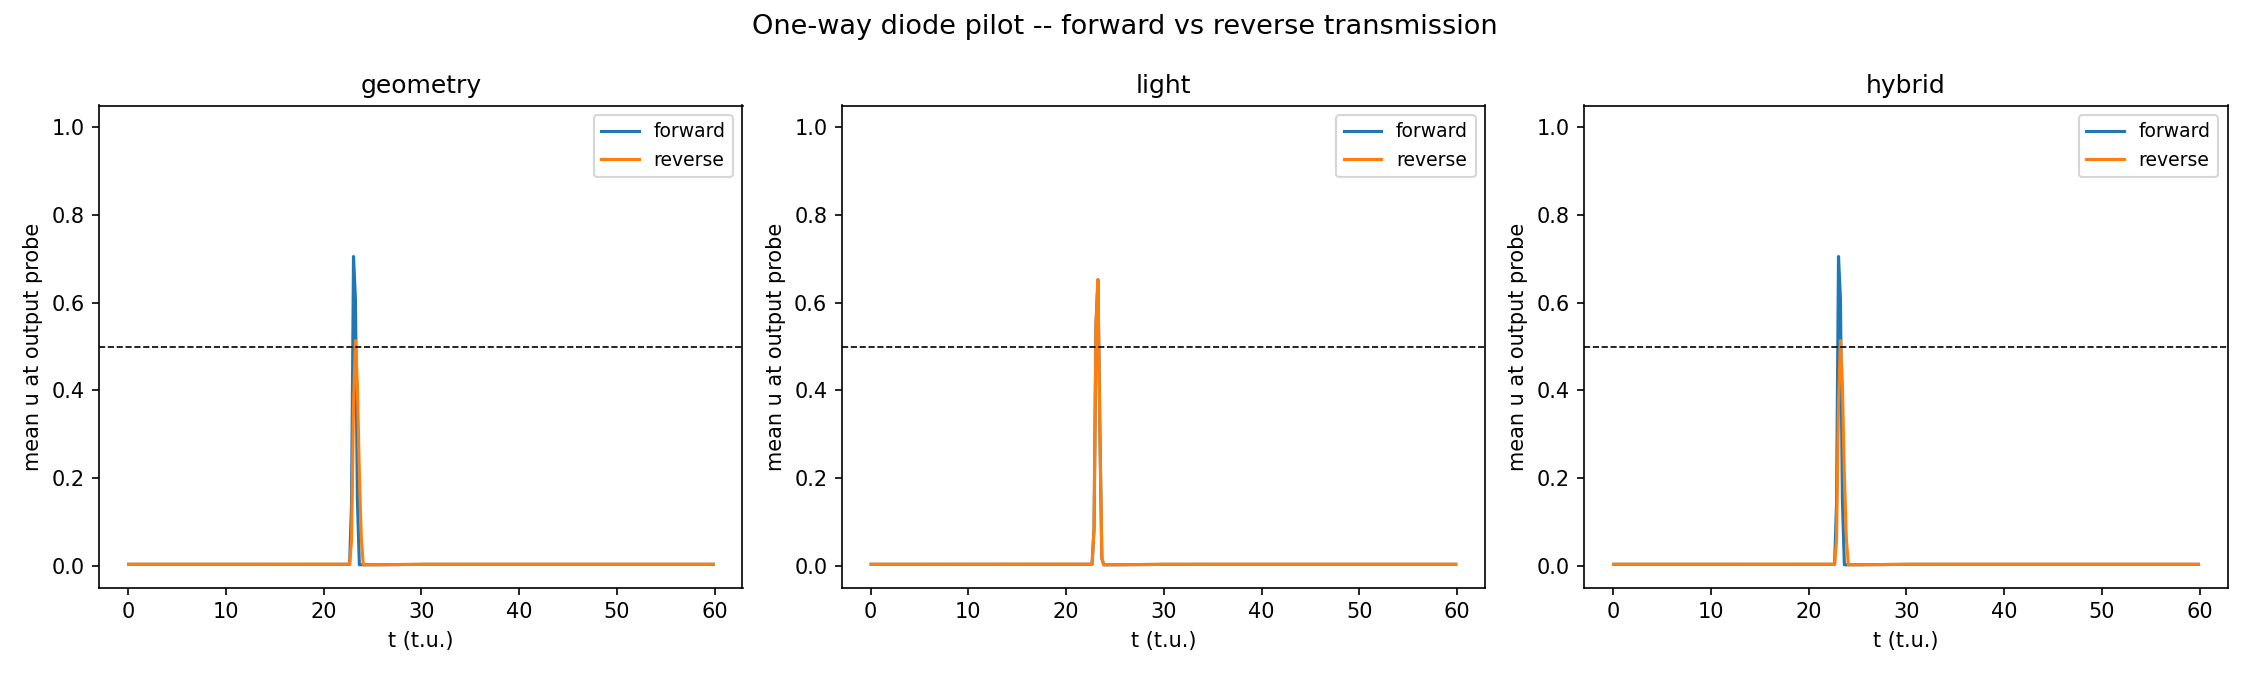
\includegraphics[width=0.95\textwidth]{../Analysis/figures/rd_diode_pilot_series.png}}{%
[figure pending]}
\caption{One-way diode pilot. Asymmetric wall geometry, a static light barrier, and a hybrid of the two all fail to give a robust forward-to-reverse extinction ratio in the present parameter regime.}
\label{fig:res_diode}
\end{figure}

\section{Uncertainty Quantification}
\label{sec:res_uq}

A one-at-a-time sensitivity analysis propagates $\pm 10\%$ uncertainty in the kinetic parameters $\varepsilon$, $f$, $\phi$, and $D_{u}$ to the channel pulse speed and amplitude.
The parameter $f$ dominates the probe peak amplitude, while $\varepsilon$ dominates the pulse speed; $\phi$ and $D_{u}$ have smaller but non-negligible effects.
This gives the characterisation a robustness layer and identifies which parameters must be constrained most tightly in any future experimental realisation.

\begin{figure}[htbp]
\centering
\IfFileExists{../Analysis/figures/pub/pub_sobol_indices.png}{%
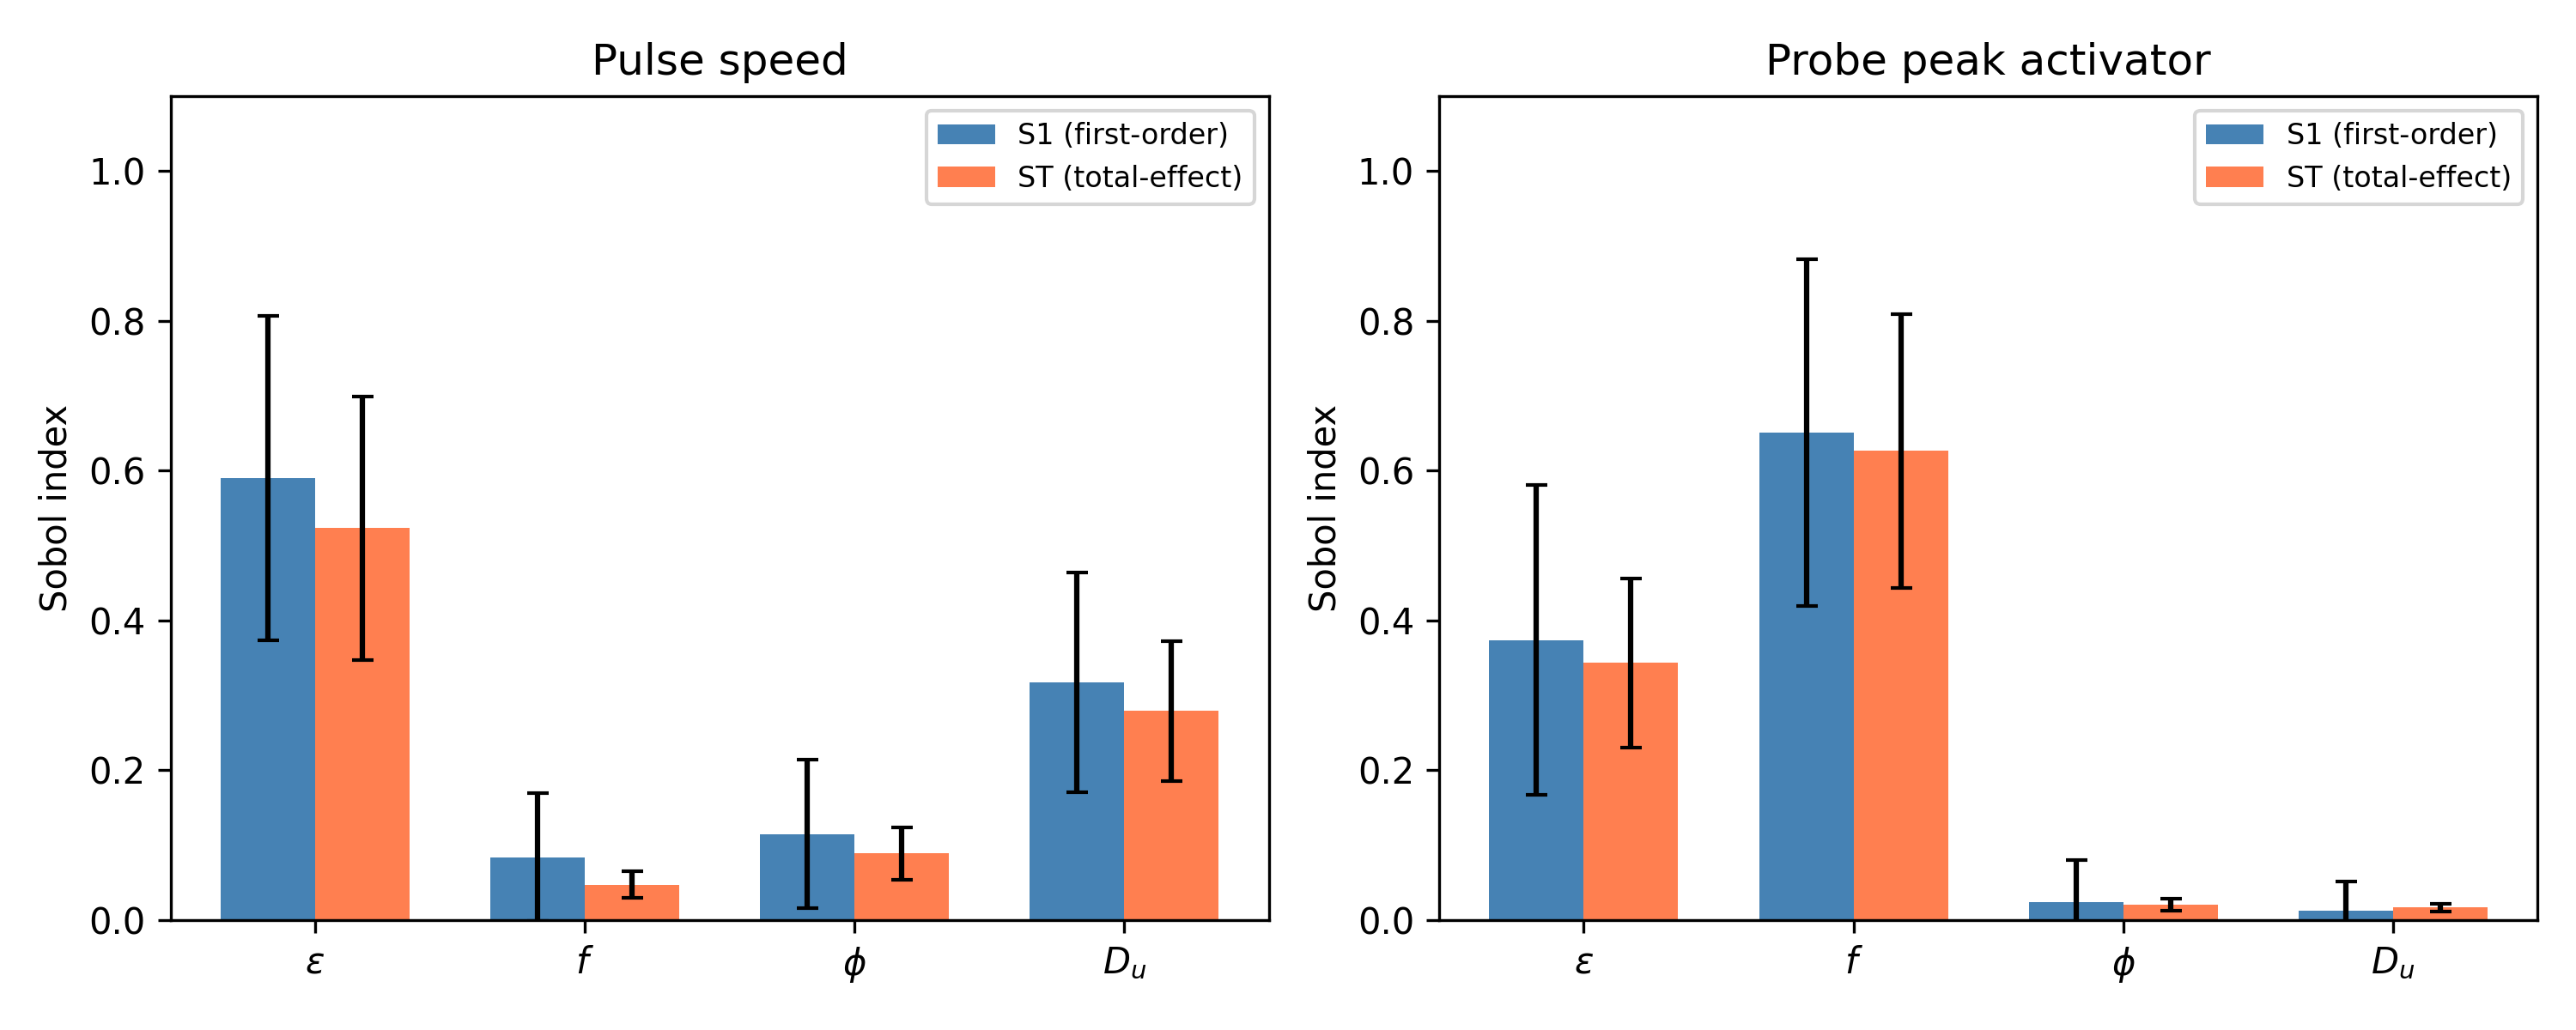
\includegraphics[width=0.9\textwidth]{../Analysis/figures/pub/pub_sobol_indices.png}}{%
[figure pending]}
\caption{One-at-a-time sensitivity of the channel pulse speed and amplitude to $\pm 10\%$ uncertainty in the kinetic parameters. $f$ dominates the amplitude and $\varepsilon$ dominates the speed.}
\label{fig:res_uq}
\end{figure}

\section{Training Attempt}
\label{sec:res_train}

A trainable light-field T-junction directionality task was attempted as a proof of concept.
A $4 \times 4$ bilinear interpolation grid parameterised $\phi(x,y)$ around the junction, and CMA-ES was used to minimise a soft loss that rewards high response at the assigned output and low response at the wrong output.
The task returned a negative result: no trainable improvement over a uniform-phi baseline was found within the optimisation budget.
This marks the practical limit of simple light-field modulation in the present regime and reinforces the characterisation-first framing: the native operators constrain what a training loop can achieve.


\chapter{Conclusions and Future Work}
\label{chap:conclusions}
% Chapter: Conclusions and Future Work

\section{Summary of Contributions}
\label{sec:conc_summary}

This thesis treated a structured Belousov--Zhabotinsky reaction--diffusion medium as the micro-scale picture inside a macro-scale porous chemical reactor.
The reactor's void space was abstracted as a pore-network graph: bulbous pores become nodes and narrow throats become edges.
The central claim was that the local pulse-traffic rules at each graph element can be measured in controlled two-dimensional simulations and then composed into a fast predictor of network-level behaviour.

Four local operators were isolated and quantified.
A straight throat is a near-perfect wire: the pulse speed is set by the kinetics and is almost independent of channel width.
Refractoriness limits the maximum signalling frequency; for the Oregonator working point used here, the absolute refractory period is 3.0 time units and the maximum one-to-one following rate is 0.167 per time unit.
A T-junction implements two-input inhibition when the readout is windowed in time: A AND (NOT B) was obtained with a separation ratio above $200\times$.
An anisotropic diffusion tensor steers pulses along preferred directions with a speed ratio that follows the eikonal $\sqrt{r}$ law.

These operators were encoded in an event-driven graph simulator.
The simulator correctly predicted the behaviour of an inhibition gate and a priority router, and it produced the correct truth table for a shared-control multi-junction gate.
Where it failed, the failure was instructive: a shared channel introduced crosstalk between two data paths that single-junction measurements did not capture, and a chambered Y-junction intended as a collision XOR leaked because the collision geometry allowed re-ignition of the output stem.
A thin-slab three-dimensional inhibition gate showed that the same operators transfer once the junction shape is corrected, and a one-way diode pilot showed that a simple asymmetric wall or static light barrier is not enough for robust rectification.
A light-field training attempt returned a negative result: within the optimisation budget, no improvement over a uniform suppression field was found.

The work therefore supports the following conclusion: network-level pulse routing in a structured excitable medium can be predicted from micro-scale transfer functions, but only when the geometry of every junction is carried explicitly in the model.
The graph abstraction is viable as a design layer between expensive continuum simulations and large network studies, but it must be calibrated against PDE solutions for each junction family.

\section{Limitations}
\label{sec:conc_limitations}

The results are limited to two-dimensional controlled simulations.
A real porous reactor is three-dimensional, and the interior light field is not known in the bulk, so the local kinetic parameters would be uncontrolled.
The 3D test reported here is a thin-slab boundary experiment, not a validated multi-gate network.

All measurements share the same computational parameter set, so the transfer functions are specific to that set.
The graph simulator uses scalar transit, refractory, and inhibition parameters extracted from idealised geometries; real junctions with rough walls, curved throats, or varying aspect ratios may require a larger library of local operators.

No experimental validation was attempted.
The mapping from model units to physical units is a calibration based on literature values, and the actual speeds and times in a wet experiment will depend on recipe, temperature, and illumination.

\section{Future Work}
\label{sec:conc_future}

The most immediate next step is to build a shape-resolved junction library.
Each entry would contain the measured transfer function for a family of junction geometries (T, Y, cross, chambered Y, angled branch), so the graph simulator can choose the right operator for each node rather than assuming a single universal value.

A second step is to incorporate uncertainty quantification into the graph simulator itself.
The one-at-a-time sensitivity analysis showed that kinetic parameters affect speed and amplitude; these uncertainties should propagate through the graph so that network-level predictions carry confidence intervals.

Third, the three-dimensional extension needs a volumetric illumination strategy.
Without a known $\phi(x,y,z)$ inside the bulk, the local operators cannot be assigned reliably.
Candidate approaches include structured light absorption, layered masks, or direct chemical patterning of the catalyst distribution.

Fourth, training should be reframed around geometry rather than around a small light-field grid.
The negative training result suggests that the native operators at the chosen working point are too stiff for small local modulation of the suppression field to change the routing decision.
Trainable porous processors may need trainable wall shape, catalyst patterning, or a richer parameterisation of the light field.

Finally, the framework should be tested against experimental data from a photosensitive BZ layer or a microfluidic excitable-medium network.
That would close the loop between the measured transfer functions and the pore-network graph, and would show whether the abstractions introduced here survive the noise and heterogeneity of a real chemical substrate.


%% --- BACK MATTER --- %%
\renewcommand{\bibname}{References}
\bibliographystyle{vancouver}
\bibliography{references}

\appendix
\chapter{Additional Derivations}
\label{app:derivations}
All derivations, model equations, and convergence data required to reproduce the reported transfer functions are presented in the main chapters. No supplementary derivations are needed.

\end{document}
